
\documentclass[preprint,12pt]{elsarticle}

\usepackage{amsmath,amssymb}
\usepackage{graphicx}
\usepackage{booktabs}
\usepackage{xcolor}
\usepackage{microtype}
\usepackage{multirow}
\usepackage{array}
\usepackage{placeins}
\usepackage{dblfloatfix}
\usepackage[T1]{fontenc}
\usepackage{lmodern}
\usepackage{url}

\renewcommand{\arraystretch}{1.1}
\setlength{\tabcolsep}{4pt}
\newcommand{\bst}{\rlap{$^{*}$}}

\begin{document}

\begin{frontmatter}

\title{Proxy-Based Urban Change Prediction under Spatial Generalization: Improving Tail Reliability with Lightweight Calibration}

\author[1]{Winston Huang\fnref{orcid}}
\ead{cnhuangwenqin@gmail.com}

\affiliation[1]{organization={Olive Tree International Academy, BFSU},
               city={Hangzhou},
               country={China}}

\fntext[orcid]{ORCID: 0009-0004-4113-8599}

\begin{abstract}
Predicting urban change from gridded Earth-observation proxies is increasingly important for urban monitoring, infrastructure assessment, and spatial decision support, but the hardest cases are not average fluctuations. They are rare local shocks, which make remotely sensed proxy targets such as $\Delta$WorldPop and $\Delta$VIIRS strongly long-tailed. Existing results can therefore be misleading for two reasons: row-wise splitting often overstates performance through spatial leakage, and average metrics understate failure in the tails, where monitoring risk is concentrated. Using CivitasGrid-TLP (2015--2024), we study long-tail spatial regression under leakage-aware GroupSplit(\texttt{grid\_id}) and benchmark multiple tabular regressors together with two tail-oriented strategies: routing-based Mixture-of-Experts (MoE) and a lightweight post-hoc affine calibrator trained with an RMSE-anchored contrastive objective. The findings are clear. $\Delta$WorldPop is consistently more predictable than $\Delta$VIIRS, whose year-to-year differencing amplifies observational noise and leaves weak signal under realistic spatial generalization. Tail errors dominate the practical difficulty of the task. The anchored calibrator consistently improves tail reliability with minimal trade-off in overall fit across diverse baselines, whereas a two-expert MoE becomes less stable and underperforms under spatial generalization. These results highlight a practical lesson for applied remote sensing: when urban proxy mapping is transferred to unseen grids, lightweight calibration can improve reliability more effectively than adding routing complexity.
\end{abstract}

\begin{keyword}
applied remote sensing \sep urban proxy dynamics \sep nighttime lights \sep WorldPop \sep long-tail regression \sep spatial generalization
\end{keyword}

\end{frontmatter}



% ===================== MAIN TEXT =====================

% =====================================================
\section{Introduction}

\subsection{Remote Sensing of Urban Dynamics: Why This Matters}
Applied remote sensing is increasingly used to monitor urban change where official socioeconomic statistics are delayed, spatially coarse, or inconsistent across jurisdictions. Gridded Earth-observation products can provide spatially explicit signals of settlement intensity, population redistribution, and human activity at resolutions that are useful for urban planning and infrastructure assessment. In this setting, however, the most consequential errors are rarely concentrated in the average case. They occur when models miss abrupt local changes such as rapid expansion, stagnation, or decline in a small number of grid cells. For operational urban monitoring, reliability on these high-impact cells is therefore more important than small gains on already easy-to-predict regions.

\subsection{The Challenge of Long-tail Remote-Sensing Proxy Dynamics}

In this study, we examine year-to-year prediction of urban proxy dynamics at the grid level using $\Delta$WorldPop and $\Delta$VIIRS as targets. Both variables are derived from widely used remote-sensing products and are strongly long-tailed: most grids remain near zero from one year to the next, while a minority experience disproportionately large shifts. This distribution is not a minor nuisance. It defines the deployment setting. Rare shocks dominate both practical monitoring risk and model error, yet standard regression pipelines are typically tuned to improve average fit rather than tail reliability.

This setting exposes two gaps in current practice. First, reported performance can be overly optimistic when evaluation allows the same spatial units to appear in both training and test sets. In grid-based panel data, row-level random splitting can leak location-specific regularities across folds, inflating apparent generalization. For remote-sensing applications, this means a model may appear strong simply because it has effectively seen the same spatial footprint before. Second, even when overall metrics look acceptable, they can conceal systematic failure in the tails, where prediction quality matters most for identifying unusual urban change. A realistic study of urban proxy dynamics therefore needs both leakage-aware spatial evaluation and metrics that explicitly examine tail behavior.

Large-scale proxy data make this problem tractable. Official statistics are often delayed, spatially coarse, or inconsistent across regions, whereas WorldPop and VIIRS provide scalable signals for fine-grained urban monitoring from remotely sensed observations. At the same time, differencing these proxies introduces additional observational noise, especially for VIIRS nighttime lights, making realistic benchmarking essential rather than optional.

\subsection{Research Questions and Overview}

Our goal is not to claim a fundamentally new predictive model class, but to resolve a practical mismatch between reported performance and real-world reliability in remote-sensing-enabled urban monitoring. Using CivitasGrid-TLP, we benchmark strong tabular regressors for long-tail spatial regression under GroupSplit(\texttt{grid\_id}), a leakage-aware protocol that tests spatial generalization to unseen grids. This benchmark is paired with tail-focused evaluation so that average accuracy and rare-event reliability can be assessed together rather than conflated.

Within this framework, we study two complementary questions. The first is whether increasing model complexity through a two-expert Mixture-of-Experts improves long-tail prediction under realistic spatial splitting. The second is whether a lightweight post-hoc calibration layer can better align predictions with tail behavior without materially degrading overall fit. To answer the latter, we introduce an RMSE-anchored contrastive affine calibrator that is model-agnostic, plug-and-play, and applicable to strong non-differentiable tabular regressors such as tree ensembles. In remote-sensing terms, the question is whether reliability on rare urban change events is better improved through more complex routing or through better calibration of already informative predictors.

A central question of this paper is whether tail robustness in spatial long-tail regression is better addressed by routing-based decomposition or by lightweight post-hoc calibration under leakage-aware spatial evaluation. Our results favor the latter: the naive MoE does not rescue tail performance and introduces additional instability, whereas the anchored calibrator delivers more reliable tail behavior with minimal cost to overall accuracy. This makes the proposed framing especially relevant to applied remote sensing, where robust transfer to new geographic locations is often more valuable than marginal gains under permissive evaluation.

This work does not aim to propose a fundamentally new predictive model class. Instead, it focuses on identifying a practical mismatch between evaluation protocols and deployment conditions in spatial proxy prediction, and provides a lightweight, model-agnostic correction strategy supported by systematic empirical evidence. We position this work as: (1) a leakage-aware evaluation benchmark, (2) a tail-focused empirical study, and (3) a practical calibration approach.

\subsection{Our Contributions}
\begin{itemize}
    \item \textbf{Leakage-aware benchmark for long-tail urban dynamics:} We formulate grid-level prediction of $\Delta$WorldPop and $\Delta$VIIRS as a long-tail spatial regression problem for remote-sensing proxy monitoring and evaluate it under GroupSplit(\texttt{grid\_id}), reducing optimistic bias from spatial leakage and better matching deployment to unseen grids.

    \item \textbf{Systematic tail-focused evaluation:} We benchmark multiple strong tabular regressors using both overall and tail-specific metrics, showing that realistic spatial generalization is substantially harder than random-split performance suggests and that $\Delta$VIIRS is markedly less predictable than $\Delta$WorldPop under year-to-year remote-sensing differencing.

    \item \textbf{Lightweight model-agnostic calibration:} We propose an RMSE-anchored contrastive affine calibrator that can be attached post hoc to diverse regressors, including non-differentiable tabular models. The method consistently improves tail reliability with only minimal trade-off in overall metrics, which is attractive for operational remote-sensing workflows.

    \item \textbf{Actionable negative result on model complexity:} We show that a two-expert MoE does not improve this task under leakage-free evaluation, indicating that in long-tail spatial settings, added routing complexity does not automatically translate into better reliability for urban Earth-observation products.
\end{itemize}

Next, we review prior work on long-tail regression, mixture-of-experts learning under heterogeneity, and remote-sensing-based proxy indicators, which together motivate our benchmark setting.

% =====================================================
\section{Literature Review}
\subsection{Long-tail Regression}

Traditional MSE/MAE-based regression models typically emphasize head (majority) samples at the expense of tail samples, resulting in reduced predictive accuracy on tail samples, particularly for heavy-tailed data. To address this bias, Ren et al.\ proposed a \emph{Contrastive Balanced MSE} approach that improves model performance on long-tailed and imbalanced samples~\cite{ren2022balancedmse}. This method not only optimizes the distance between $\hat{y}_i$ and $y_i$, but also maximizes the distance between $\hat{y}_i$ and other samples' $y_j$, effectively reducing the dominant influence of head samples during training. Similarly, Yang et al.\ proposed \emph{Deep Imbalanced Regression}~\cite{yang2021dir}, which combines \emph{Label Distribution Smoothing} (LDS) and \emph{Feature Distribution Smoothing} (FDS) to improve generalization under heavy-tailed targets. These complementary approaches motivate our setting, where long-tailed proxy dynamics interact with heterogeneous regional mechanisms and routing-based models.

\subsection{Mixture-of-Experts}

Yuksel et al.\ reviewed two decades of Mixture-of-Experts (MoE) research and applications~\cite{yuksel2012twenty}. Their work suggests that when data involve multiple regimes with heterogeneous mechanisms, a single model may be insufficient, but MoE with a soft routing gating network can substantially improve model fit by assigning each input to one or multiple experts. MoE can significantly improve fitting ability under heterogeneity; however, residual spikes may emerge when gating decisions are unstable.

While Yuksel et al.\ provide an overarching view of MoE as a divide-and-conquer framework, subsequent work formalizes MoE as a conditional mixture model. In Gormley and Frühwirth-Schnatter's research, MoE is formulated as a conditional mixture model where both mixing weights ($\pi_k$) and expert distribution parameters depend on covariates~\cite{gormley2018moe}. MoE can model heterogeneity and subgroup structure effectively; however, the stability of MoEs depends critically on the smoothness and identifiability of the gating model.

Building on this statistical formulation, recent surveys highlight how MoE has been adapted to diverse learning tasks including regression under heterogeneous conditional distributions. Nguyen and Chamroukhi provide a comprehensive overview of MoE variants across regression, classification, and clustering~\cite{nguyen2018overviewmoe}, systematically reviewing hierarchical MoE, mixture of linear experts, time-series mixtures, and mixture-of-regression models with gating networks. Through this review, they emphasize that gating routing (soft vs.\ hard) and gating-model complexity influence stability and interpretability. In our work, we implement a hierarchical MoE approach that divides head and tail into two separate regimes, each handled by a mixture of two experts.

Beyond point prediction, recent work explores distributional regression using MoE-based approaches, which is particularly relevant for heavy-tailed targets. Rügamer et al.\ propose an innovative approach for processing long-tailed and heavy-tailed data with outliers and shocks~\cite{rugamer2024mixdistreg}. Rather than predicting $\mathbb{E}[Y|X = x]$, distributional regression models predict the full conditional distribution $Y|X=x$, which significantly enhances robustness and reliability. However, in practice, long-tail regression benchmarks often use target transformations and gating-based experts, which can suffer from boundary-induced residual spikes due to uncertain routing and transformation inversion.

Overall, existing MoE literature establishes the framework as a powerful strategy for learning heterogeneous regimes, and recent distributional extensions highlight its potential for robustness under heavy-tailed targets. However, most studies focus on modeling flexibility, inference, and application-level performance, leaving a gap in systematically characterizing and mitigating stability issues in long-tail regression. Specifically, when gating decisions are uncertain near boundaries and expert predictions are limited under different target transformations, small differences can be amplified, leading to boundary-induced residual spikes and unacceptable worst-case errors. Motivated by this gap, our work empirically investigates stable MoE strategies under heavy-tailed proxy prediction and proposes an evaluation benchmark.

\subsection{Proxy-based Socioeconomic Indicators}
Beyond modeling strategies, our task depends on scalable, high-resolution proxies of economic dynamics, since official statistics are often unavailable at the grid level.

For population as an economic indicator, Paganelli notes that Adam Smith recognized population growth as a proxy for economic growth~\cite{paganelli2021populationgdp}: if a region can support population growth, its productivity is likely also increasing. Population change reflects aggregate outcomes of resource availability, labor demand, and wage dynamics rather than noise, providing meaningful signals for interpreting economic booms and recessions. This historical perspective validates our use of population-density data (WorldPop) when high-resolution official GDP data are unavailable. Peterson further emphasizes that population growth impacts vary by development level: in low-income economies it may dilute capital, while in high-income economies it can enable specialization~\cite{peterson2017rolepopulation}. This heterogeneity motivates training specialized experts for different development contexts.

Regarding nighttime luminosity as an economic proxy, Chen and Nordhaus demonstrate that nighttime light intensity is an objective, globally-available, spatially high-resolution indicator that can be used to replace or supplement traditional economic statistics~\cite{chen2011luminosity}. Their systematic analysis of GDP and luminosity across 12,393 globally distributed $1^{\circ} \times 1^{\circ}$ grid cells (1992--2008) found a notably strong correlation ($R^2 = 0.97$) between illuminated area and GDP, validating VIIRS Nighttime Light Intensity as a proxy for economic dynamics. However, at finer spatial scales, the relationship becomes noisier and less reliable, especially in low-output regions. Measurement error in log-luminosity across satellites introduces substantial uncertainty (SE 0.28--0.59), corresponding to $\ge 25\%$ proxy error. Thus, a more robust long-tail prediction model is essential.

Prior work primarily uses population or luminosity to approximate static economic output levels, but urban planning often requires predicting changes rather than absolute levels. This motivates defining targets as year-to-year differences rather than absolute values.

\subsection{Literature Review Summary}

In summary, prior work validates the use of population and nighttime luminosity as scalable remote-sensing proxies of urban and economic activity and extensively explores MoE for learning under heterogeneity. Long-tail regression research shows that standard MSE/MAE training biases models toward head samples, and remedies such as Balanced MSE and distribution smoothing (LDS/FDS) can improve tail performance under heavy-tailed targets. However, existing studies rarely provide unified benchmarks for grid-level proxy dynamics prediction that simultaneously reflect remote-sensing observation noise, transportation morphology features, long-tailed targets, and leakage-aware evaluation. To address this gap, we introduce CivitasGrid-TLP as a benchmark dataset and investigate robust long-tail modeling strategies with controlled MoE and contrastive learning frameworks.



% =====================================================
\section{Dataset: CivitasGrid-TLP}

CivitasGrid-TLP is a grid-level panel dataset designed for proxy-based urban dynamics prediction from heterogeneous geospatial observations~\cite{huang_2026_18144416}. It integrates transportation network features and remotely sensed proxy signals (WorldPop population density and VIIRS nighttime light) across thousands of city grids (30''--60'' resolution), supporting an applied remote-sensing view of urban change monitoring rather than a purely tabular benchmark.

\subsection{Data Sources and Grid Definition}

We define the basic spatial unit as a grid cell (30"–60"), and constructed a panel dataset spanning 2015–2024. Each grid-year record links a spatial cell with a calendar year, enabling year-to-year dynamics prediction.


\begin{table}[htbp]
    \centering

    \begin{tabular}{lccc}
        \toprule
        \textbf{Source} & \textbf{Type} & \textbf{Resolution} & \textbf{License}\\
        \midrule
         OpenStreetMap & Transportation & N/A & ODbL \\
         VIIRS V2 & Nighttime Light & 15'' & CC0 \\
         WorldPop & Population Density & 1 km & CC BY \\
        \bottomrule
    \end{tabular}
    \caption{Data sources and specifications}
    \label{tab:datasources}
    
\end{table}


As shown in Table~\ref{tab:datasources}, we extracted transportation features from OpenStreetMap and linked them with proxy signals including VIIRS nighttime light intensity and WorldPop population density. Unlike existing work, which typically focuses on coarse administrative regions, CivitasGrid-TLP provides a grid-based benchmark at kilometer-level resolution, supporting remote-sensing-oriented evaluation across regions and countries.


\subsection{Targets and Feature Groups}

Model inputs in CivitasGrid-TLP are organized into three groups: (i) transportation network features, (ii) lagged proxy levels, and (iii) categorical descriptors. Transportation features are derived from OpenStreetMap (OSM) and aggregated into seven morphology categories capturing road density, hierarchy, and intersection structure. To ensure comparability across grids of different spatial resolutions, all OSM-derived features are normalized by grid area (per km$^2$). When OSM coverage is absent or insufficient, transportation features are set to zero, indicating unmapped road infrastructure.

For proxy signals, we include previous-year absolute levels of WorldPop population density and VIIRS nighttime light intensity as minimal temporal context. The prediction targets are year-to-year changes: $\Delta$WorldPop and $\Delta$VIIRS, which emphasize local dynamics while reducing baseline-level heterogeneity across regions.

Finally, categorical descriptors including country code, city type, and functional zone characterize heterogeneous regional contexts and enable stratified evaluation across development regimes.



\subsection{Data Definition and Calculation}

We define the prediction task as grid-level, year-to-year dynamics forecasting of proxy economic signals. Given features and lagged proxy observations for a grid cell, the goal is to predict proxy signal changes from year $t-1$ to year $t$.

Specifically, we forecast two targets: population density change ($\Delta$WorldPop) and nighttime light change ($\Delta$VIIRS), defined as:
\begin{equation}
    \Delta \text{WorldPop} = \text{WorldPop}_t - \text{WorldPop}_{t-1}
\end{equation}
\begin{equation}
        \Delta \text{VIIRS} = \text{VIIRS}_t - \text{VIIRS}_{t-1}
\end{equation}

Differencing captures local urban dynamics and reduces baseline differences across regions. Most grid cells experience minor year-to-year fluctuations, while a non-negligible subset undergoes abrupt shocks. From a remote-sensing perspective, these differenced products emphasize change detection but also amplify sensor- and preprocessing-related noise, which motivates strategies prioritizing tail and worst-case performance.

\subsection{Quality Control and Filtering Tiers}

Given substantial variation in data quality and completeness across regions and time, we adopt a tiered filtering procedure to construct subsets with different quality–coverage trade-offs. Transportation features are grouped into seven feature categories. For each grid-year record, we count available (non-missing) OSM feature categories.

We define two filtering tiers based on transportation feature completeness. Records with fewer than three available OSM feature categories are excluded due to insufficient information. Remaining records form the Medium-Quality (MQ) dataset. A stricter High-Quality (HQ) dataset is further defined by retaining records with at least four available OSM feature categories. This tiered design enables systematic evaluation under different quality constraints while maintaining transparency and reproducibility. We begin with 7,500 candidate grids. To focus on economically meaningful urban dynamics and exclude extremely sparse areas with limited analytical value, we first remove grids with population density below 5 km$^{-2}$. This leaves 6,178 unique grids in CivitasGrid-TLP v1.1.0. We then apply the MQ/HQ filtering criteria based on OSM feature completeness. The table below reports the resulting grid counts after each stage.
\begin{table}[htbp]
    \centering
    \begin{tabular}{lr}
        \toprule
        \textbf{Dataset Tier} & \textbf{Grid Count}\\
        \midrule
        Initial Candidates & 7,500 \\
        Population Masked & 6,178 \\
        Medium-Quality (MQ) & 4,293 \\
        High-Quality (HQ) & 2,833 \\
        \bottomrule
    \end{tabular}
    \caption{Dataset filtering results (grid counts)}
    \label{tab:filtering}

\end{table}

In the next subsection, we report the resulting sample sizes, geographic coverage, and long-tail diagnostics for the MQ and HQ subsets.


\subsection{Dataset Statistics and Long-Tail Diagnostics}

After removing candidate grids with population density below 5 km$^{-2}$, CivitasGrid-TLP v1.1.0 contains 6,178 unique grid cells observed over 10 years (2015–2024), yielding 61,780 grid-year records in total. Applying the OSM-completeness filters further retains 42,930 records in the Medium-Quality (MQ) subset and 28,330 records in the High-Quality (HQ) subset, corresponding to 4,293 and 2,833 unique grids, respectively.

The dataset covers 85 countries (HQ) or 100 countries (MQ) with diverse regional contexts, including nation code, region type, and city type as categorical descriptors. This diversity introduces heterogeneous feature distributions and motivates generalization evaluation across regions. Top 5 countries by grid count:

\begin{table}[htbp]
    \centering
    \begin{tabular}{clrr}
        \toprule
        \textbf{Rank} & \textbf{Nation Code} & \textbf{HQ Grid Count} & \textbf{MQ Grid Count}\\
        \midrule
        1 & USA & 1,715 & 2,523\\
        2 & CHN & 401 & 581\\
        3 & IND & 90 & 186\\
        4 & JPN & 87 & 120\\
        5 & CAN & 43 & 68\\
        \midrule
        Total & N/A & 2,833 & 4,293 \\
        \bottomrule
    \end{tabular}
    \caption{Geographic distribution: top-5 countries by grid count}
    \label{tab:countrycounts}
\end{table}
\FloatBarrier
\FloatBarrier
\begin{figure*}[!t]
    \centering
    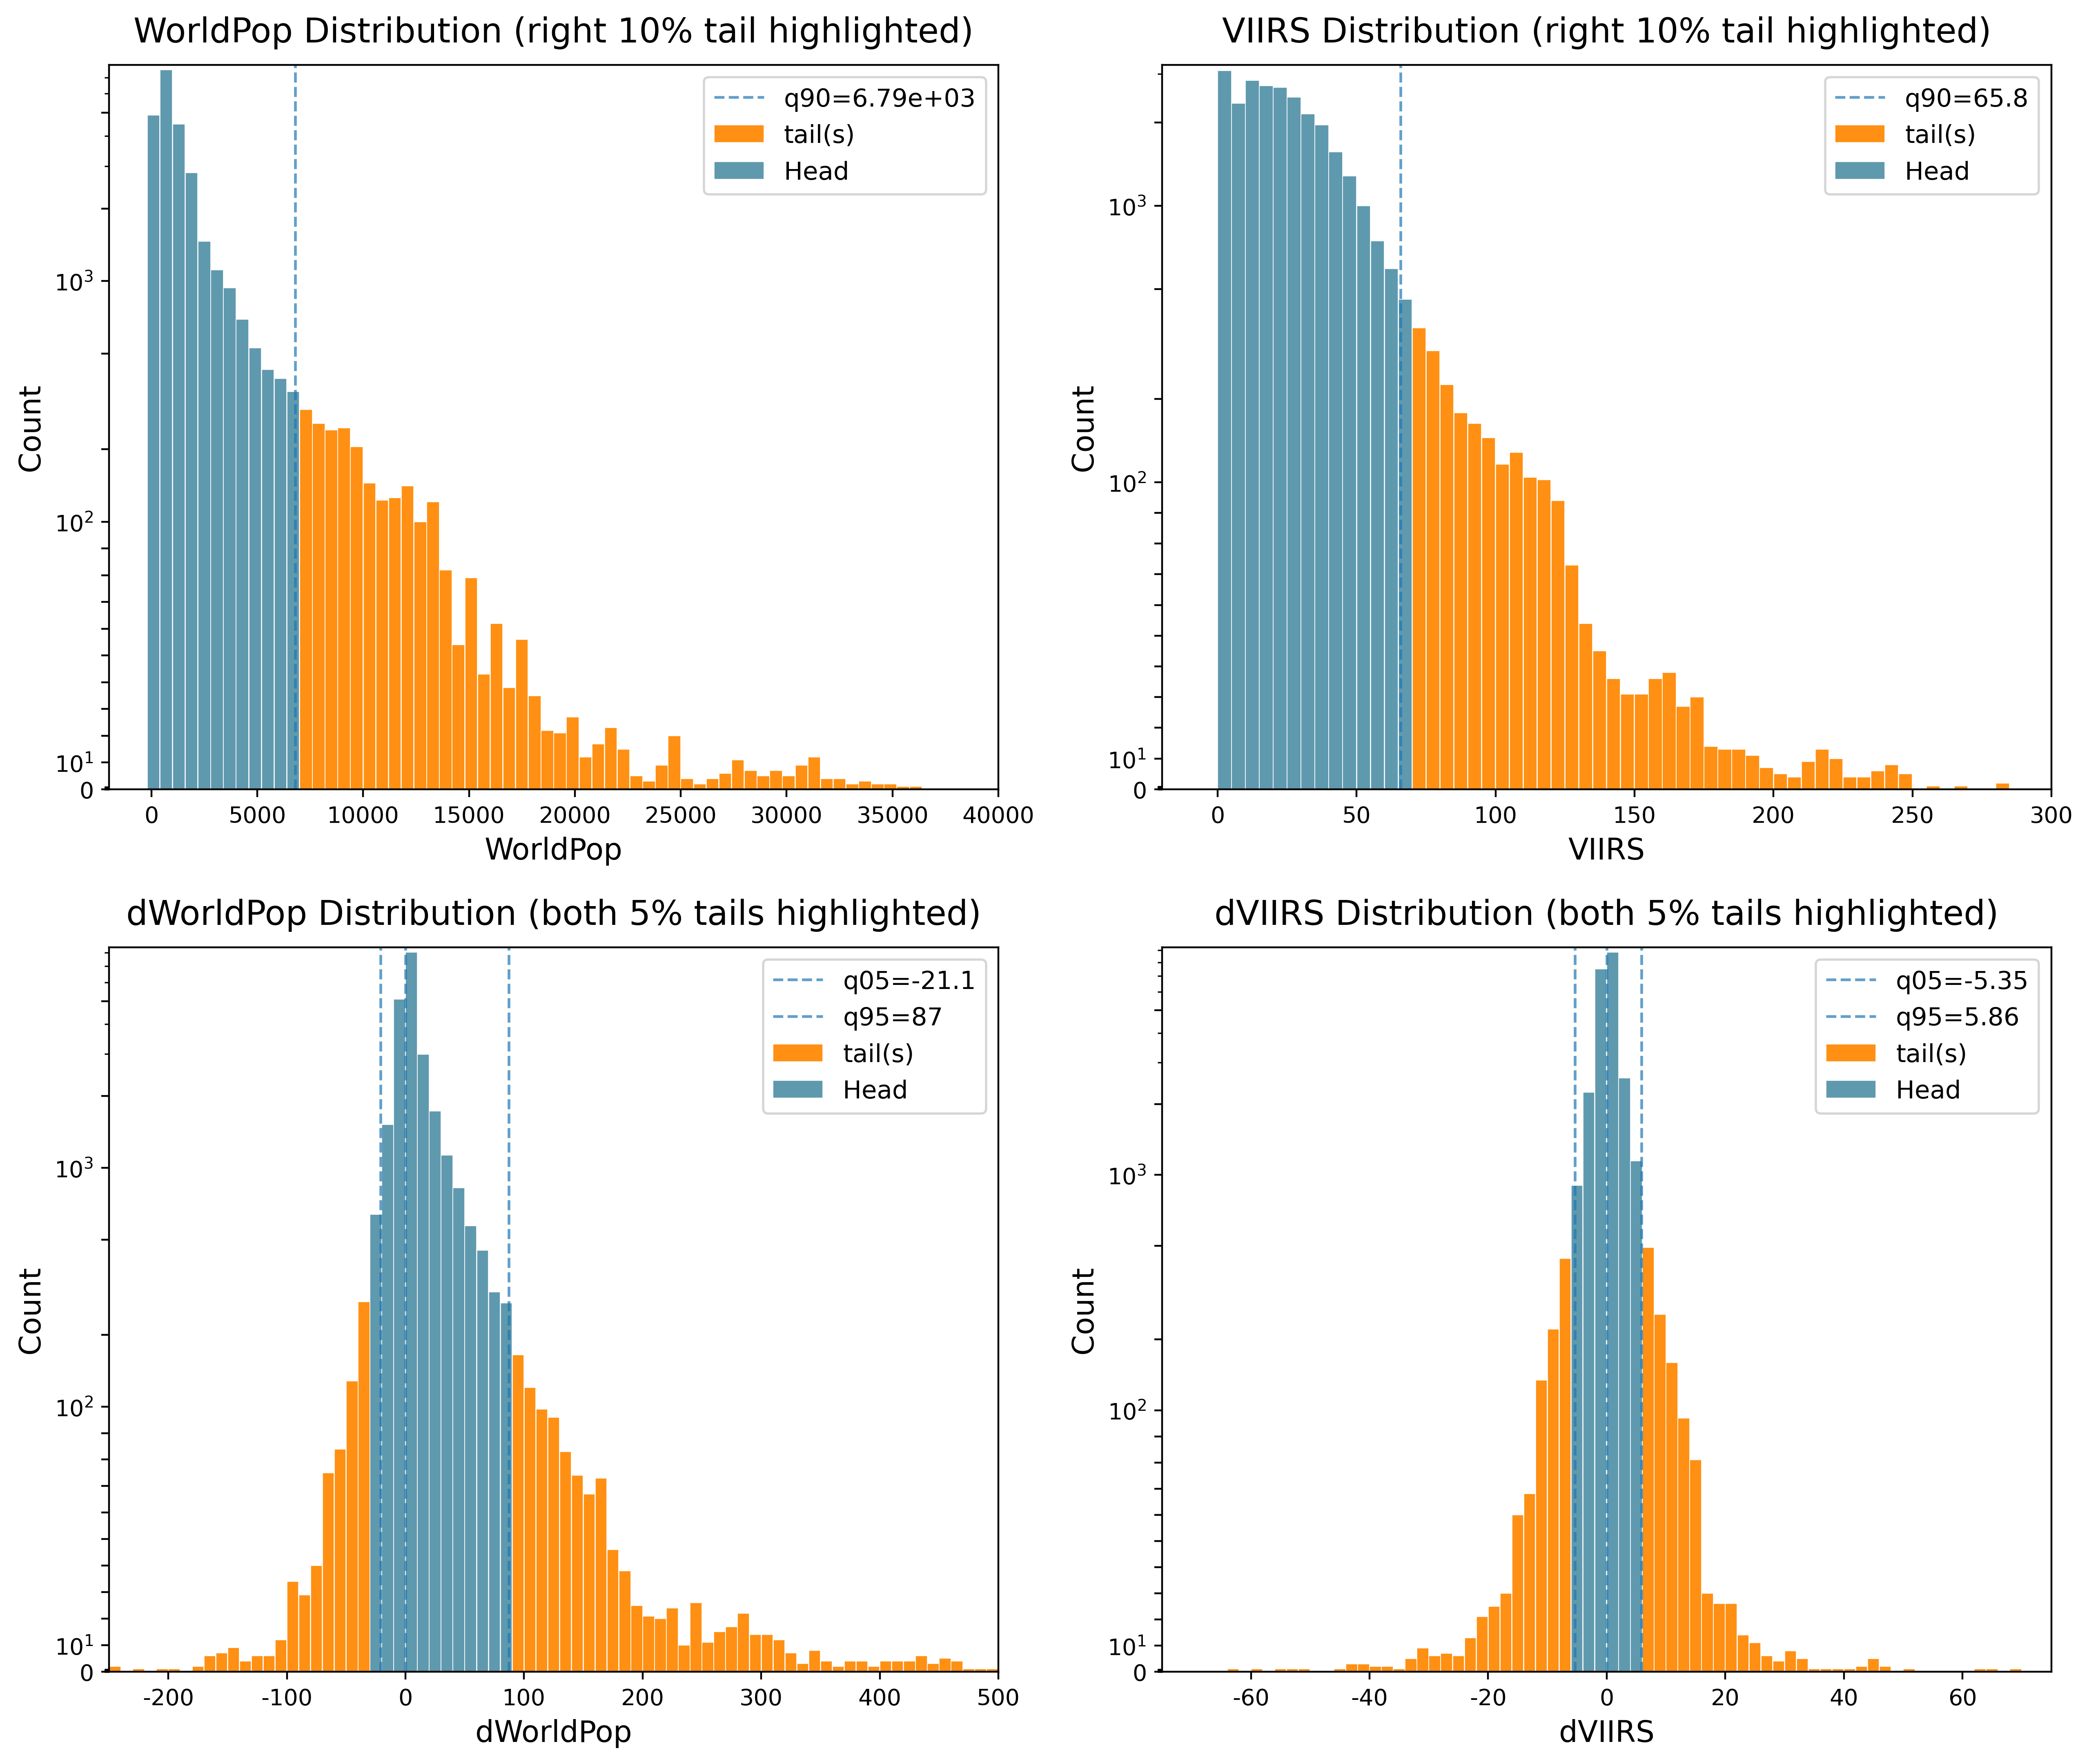
\includegraphics[width=0.9\linewidth]{figures/Distrib.png}
    \caption{Distribution of proxy signals and their year-to-year changes, illustrating the long-tailed nature of both absolute levels and changes. The y-axis uses a piecewise log scale: values below 100 are plotted linearly, while values above 100 use a logarithmic scale to reveal tail frequencies.}
    \label{fig:distribfig}
\end{figure*}

As shown in Table~\ref{tab:tgsummarystat}, both $\Delta$WorldPop and $\Delta$VIIRS exhibit high variance and strong positive kurtosis, indicating heavy-tailed dynamics with frequent small fluctuations and occasional extreme shocks.


\begin{table}[htbp]
    \centering
    \resizebox{0.47\textwidth}{!}{
    \begin{tabular}{lrrrrrrrrrrrrr}
        \toprule
        \textbf{Target} & \textbf{Mean} & \textbf{Std.\ Dev.} & \textbf{Min} & \textbf{5\%} & \textbf{25\%} & \textbf{Median}\\
        \midrule
        $\Delta$WorldPop & 16.37 & 52.54 & $-$733.6 & $-$21.10 & $-$1.258 & 4.195 \\
        $\Delta$VIIRS    & 0.190 & 4.333 & $-$63.60 & $-$5.354 & $-$1.042 & 0.100 \\
        \bottomrule
    \end{tabular}
    }
    \caption{Target summary statistics (part 1)}
    \label{tab:tgsummarystat_1}
\end{table}
\vspace{-0.4cm}
\begin{table}[htbp]
    \centering
    \resizebox{0.47\textwidth}{!}{
    \begin{tabular}{lrrrrrrrrrrr}
        \toprule
        \textbf{Target} & \textbf{75\%} & \textbf{95\%} & \textbf{Max} & \textbf{Skewness} & \textbf{Kurtosis}\\
        \midrule
        $\Delta$WorldPop & 20.60 & 86.97 & 930.9 & 5.520 & 65.96 \\
        $\Delta$VIIRS & 1.402 & 5.864 & 68.86 & 0.174 & 29.41\\
        \bottomrule
    \end{tabular}
    }
    \caption{Target summary statistics}
    \label{tab:tgsummarystat}
\end{table}

Figure~\ref{fig:distribfig} visualizes the distributions of proxy signals and their year-to-year changes for the HQ dataset. While absolute levels are right-skewed, differenced targets exhibit clear heavy-tailed patterns: most values concentrate near zero, while a substantial fraction lies far beyond. Such long-tailed targets pose challenges for average-error-optimized regression models and for remote-sensing change analysis more broadly, because rare but meaningful local anomalies are precisely the cases users care about.

\textbf{Tail and Head Split.} For each target $y$ ($\Delta$VIIRS and $\Delta$WorldPop), we define tail samples as grid-year records with absolute magnitude $|y|$ in the top $5\%$ of the empirical distribution. This symmetric definition captures both positive and negative shocks, focusing on rare high-magnitude events. We use this tail subset throughout evaluations to characterize long-tail behavior and analyze model reliability under extreme events.

\subsection{Spatial Coverage and Sampling Bias}

Figure~\ref{fig:distribmap} shows the global spatial distribution of grids in CivitasGrid-TLP. Coverage is comprehensive but nonuniform: grids concentrate in regions with well-mapped road networks and stable proxy availability (North America, Europe, East and South Asia), while sparse in low-coverage areas. This imbalance is expected for datasets combining volunteered geographic information with remote sensing.

\begin{figure}[htbp]
    \centering
    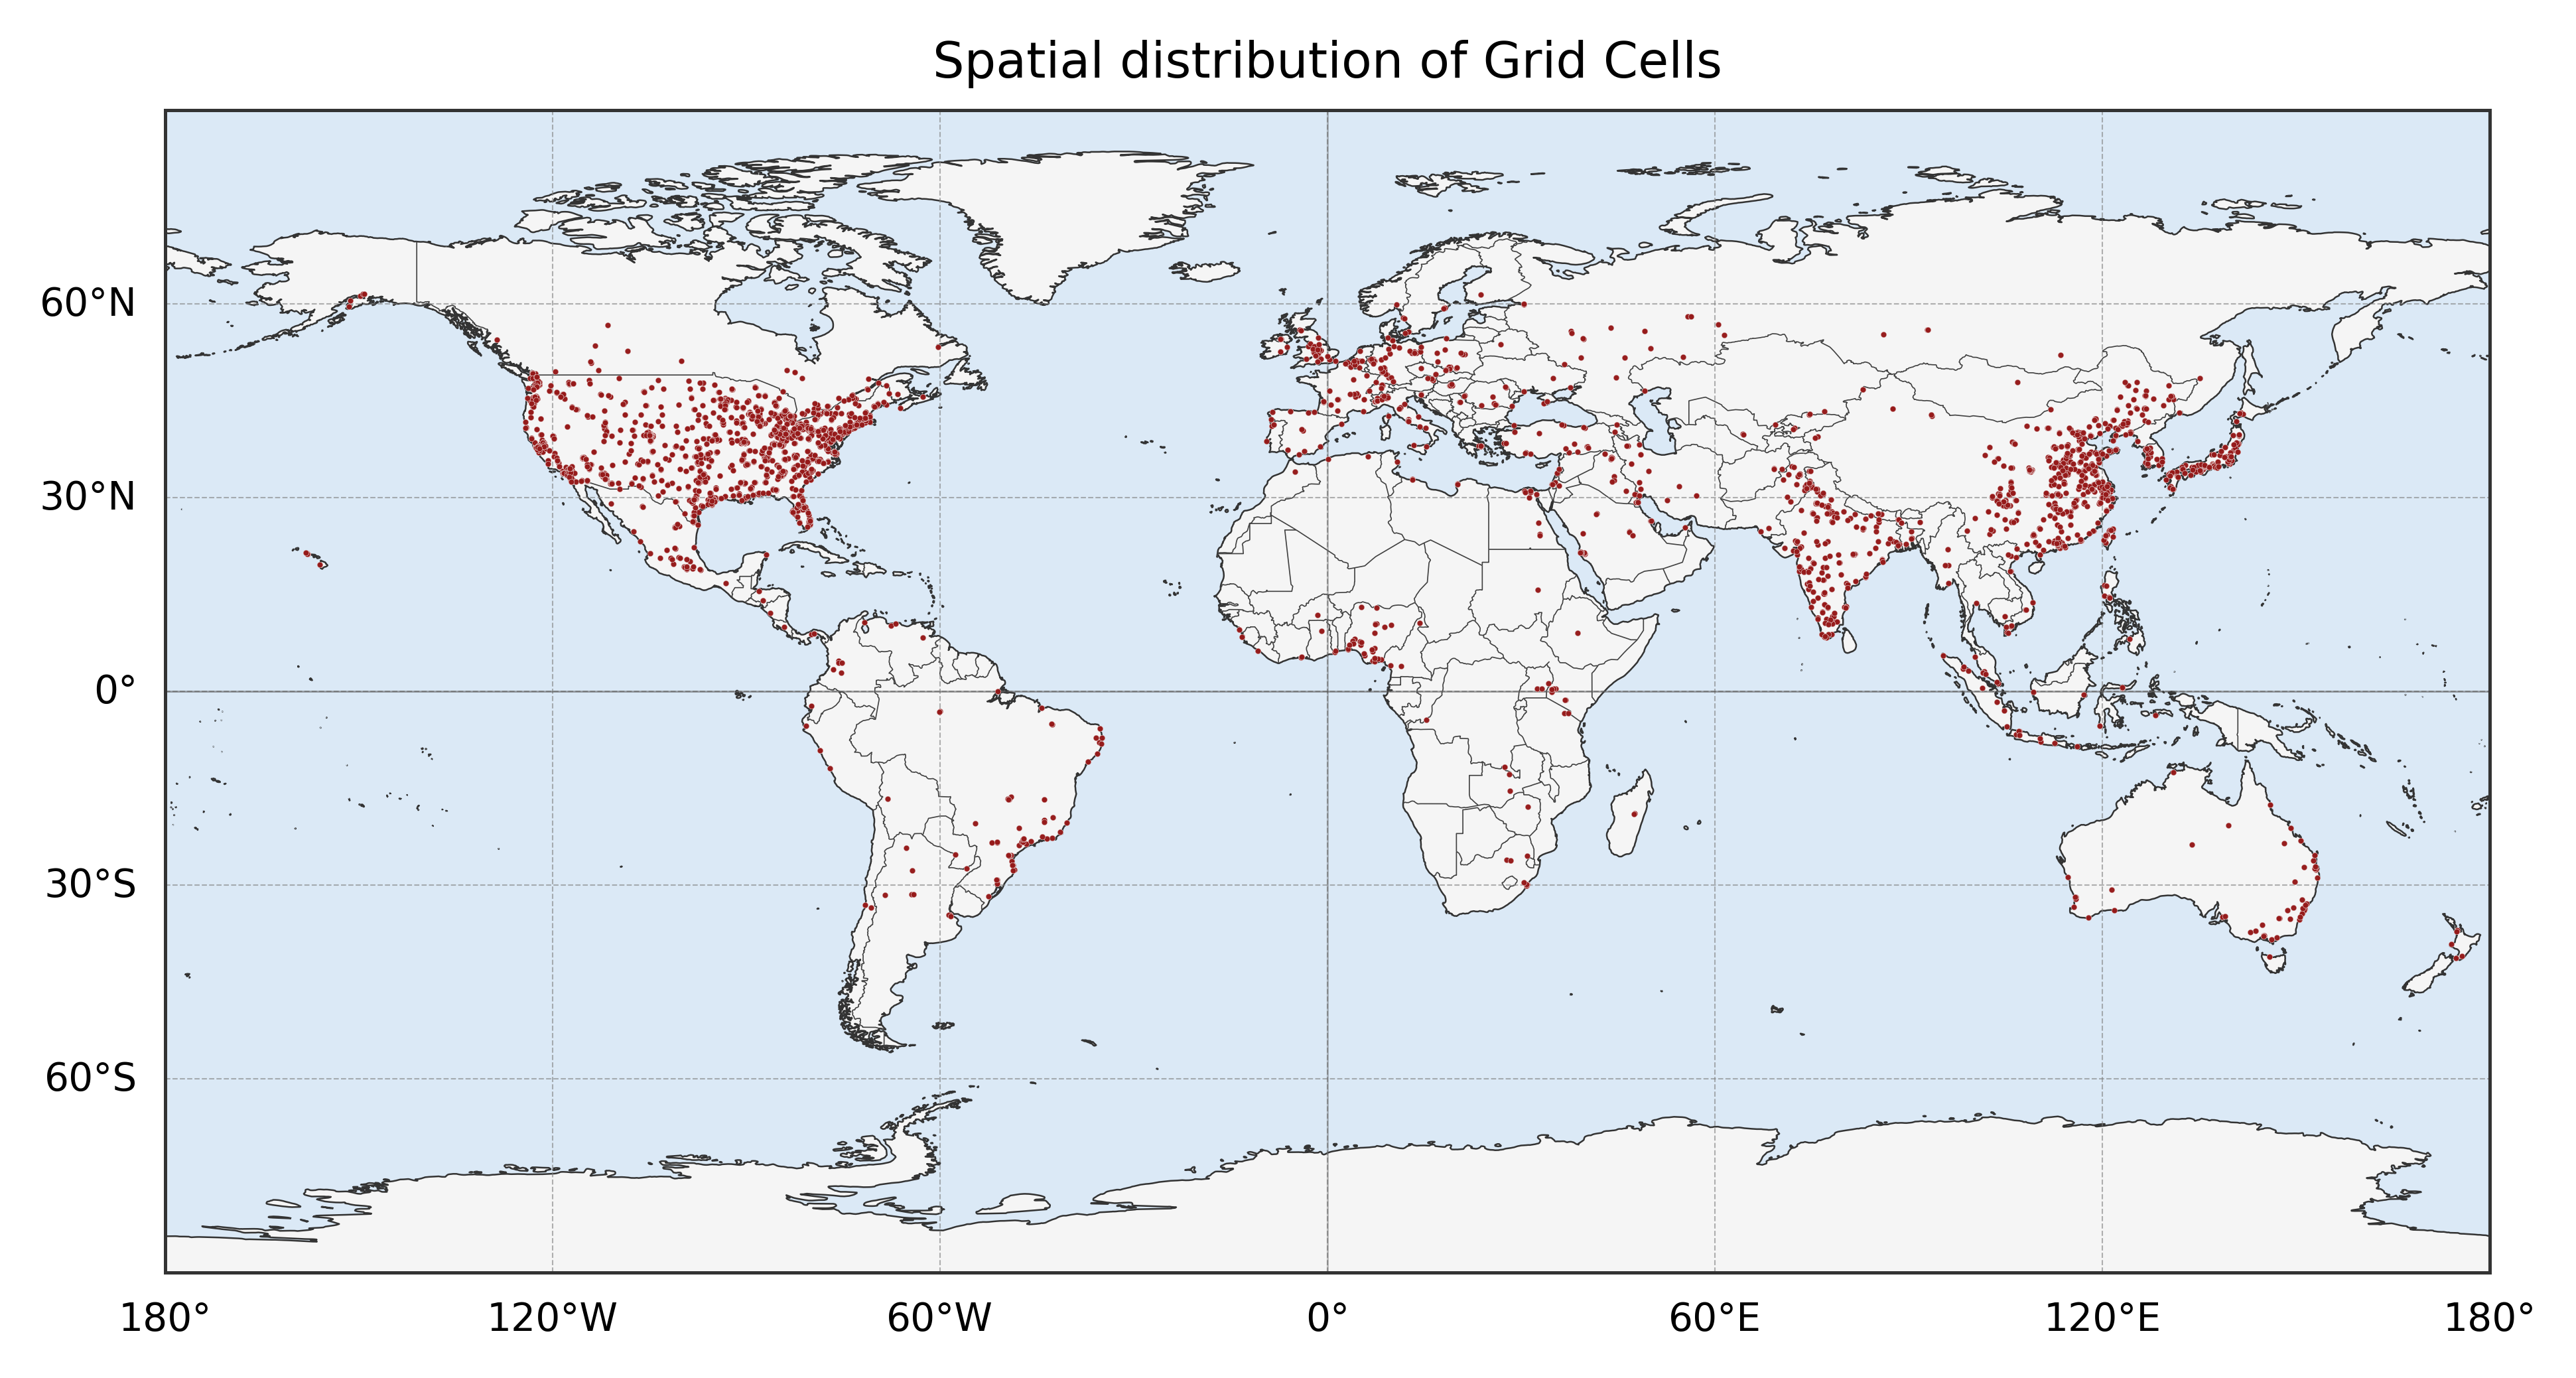
\includegraphics[width=0.9\linewidth]{figures/distrib_map.png}
    \caption{Global spatial distribution of grids in CivitasGrid-TLP, showing coverage concentration in well-mapped urbanized regions.}
    \label{fig:distribmap}
\end{figure}

Non-uniform coverage introduces sampling through two channels. First, OSM completeness varies substantially across and within countries, affecting transportation feature availability. Second, quality-control filtering further excludes records with insufficient features, implicitly favoring well-mapped urbanized regions and disadvantaging rural areas. HQ/MQ subsets therefore over-represent documented regions while under-representing rural contexts.

These long-tail and coverage challenges motivate our modeling framework and evaluation protocol.

% =====================================================
\section{Methodology}
This section introduces the benchmark baselines and our controlled experimental variants, including an objective-level contrastive learning (CL) calibration layer and a two-expert MoE design for improving tail and worst-case performance. The methodological emphasis is practical: we evaluate whether common machine-learning tools can be made more reliable for remote-sensing proxy monitoring under realistic geographic transfer.

\subsection{Problem Setup and Tail Definition}
\label{sec:problem_setup}

We evaluate two strategies for improving tail performance---Mixture-of-Experts and contrastive learning calibration---on the CivitasGrid-TLP dataset. We consider a grid-level regression problem where each sample has features $x_i$ consisting of transportation morphology, lagged proxy levels, and categorical descriptors, while the target is the year-to-year change in the proxy signal. The targets exhibit long-tailed distributions, with most samples near zero and a small but significant fraction at extreme values. In remote-sensing terms, these tail cases correspond to unusually large local deviations in the observed proxy fields. We define tail samples as those in the lower 5\% or upper 5\% of the empirical distribution:

\paragraph{Definition 1 (Tail Region).}
Let $q_{\mathrm{low}}$ and $q_{\mathrm{high}}$ denote the 5th and 95th percentiles of the training targets. We define the tail region as samples where $y < q_{\mathrm{low}}$ or $y > q_{\mathrm{high}}$.

\paragraph{Definition 2 (Tail RMSE).}
Tail RMSE is computed as the root mean squared error restricted to samples in the tail region, i.e.,
\begin{equation}
\mathrm{RMSE}_{\mathrm{tail}}=\sqrt{\frac{1}{|\mathcal{T}|}\sum_{i\in\mathcal{T}}(y_i-\hat{y}_i)^2}.
\end{equation}

\paragraph{Definition 3 (Spatial Leakage).}
Spatial leakage occurs when spatial units (\texttt{grid\_id}) appear in both training and test sets, allowing models to exploit location-specific correlations that do not generalize to unseen grids.

\paragraph{Definition 4 (Anchored Contrastive Objective).}
The calibrator is trained using a combination of RMSE loss and a contrastive loss normalized by the base model's reference scale, ensuring balanced optimization between global fit and tail discrimination. In our implementation, this reference scale is computed from the base calibrator $(a,b)=(1,0)$ on the training split.

\begin{equation}
\begin{aligned}
i\in\mathcal{T}_{\mathrm{VIIRS}} &\iff
\begin{cases}
\Delta \mathrm{VIIRS}_i \le -5.35,\\
\Delta \mathrm{VIIRS}_i \ge 5.86,
\end{cases}\\
i\in\mathcal{T}_{\mathrm{WorldPop}} &\iff
\begin{cases}
\Delta \mathrm{WorldPop}_i \le -21.1,\\
\Delta \mathrm{WorldPop}_i \ge 87.
\end{cases}
\end{aligned}
\end{equation}
where the thresholds correspond to empirical percentiles. In CivitasGrid-TLP, each sample $i$ is a \emph{grid-year} record: a fixed spatial grid at year $t$, with features from transportation morphology, lagged proxy levels, and categorical descriptors, and targets as first differences $\Delta s_{i,t} = s_{i,t}-s_{i,t-1}$ for proxy signal $s$.

To ensure reproducibility and prevent leakage, all percentile thresholds are computed on the training split only and applied unchanged to validation and test splits.

We treat $\Delta$VIIRS and $\Delta$WorldPop as separate targets with independent tail sets. In evaluation, we report overall metrics on the full set and tail-specific metrics on the subset, since our goal is improving reliability under rare high-magnitude shocks.

\subsection{Baseline Model}

We choose XGBoost as our primary baseline because it performs well on tabular data through its ability to capture nonlinearities and feature interactions. The implementation is mature, efficient, and scalable, providing stability and interpretability.

XGBoost is a regularized gradient boosting framework that builds additive decision tree ensembles by iteratively fitting new trees to negative loss gradients using second-order Hessian information.

We also include Random Forest as a non-boosting classical baseline that provides complementary performance. Additionally, we include several standard baselines (Ridge Regression, Elastic Net, SVR, Extra Trees Regressor, and MLP) in controlled experiments to ensure our conclusions are not model-specific.

\subsection{Contrastive Learning Evaluation}
\label{sec:contrastive}
We evaluate \emph{objective-level} contrastive learning (CL) as a generic tail-aware signal. Because many competitive tabular regressors are non-differentiable (e.g., random forests, SVR), we apply CL through a lightweight \emph{post-hoc affine calibration} layer that can be trained on top of \emph{any} baseline predictor.

Given a trained baseline $f(\cdot)$, we first obtain its predictions $\hat{y}^{(0)}=f(x)$. We then train an affine calibrator on the training split only:
\begin{equation}
\tilde{y} \;=\; a\,\hat{y}^{(0)} + b,
\end{equation}
and evaluate $\tilde{y}$ on the held-out test split. We consider three configurations per baseline:
\begin{itemize}
    \item \textbf{No-CL:} raw baseline prediction $\hat{y}^{(0)}$ (no calibrator);
    \item \textbf{CL-only:} calibrator trained using the contrastive objective $\mathcal{L}_{\mathrm{con}}$, denoted as \texttt{(Baseline)\_CL};
    \item \textbf{RMSE+CL (mixed):} calibrator trained using a normalized mixture of RMSE and $\mathcal{L}_{\mathrm{con}}$, denoted as \texttt{(Baseline)\_RMSE\_CL}.
\end{itemize}
This design enables a controlled comparison of objectives while keeping the underlying baseline model and data splits fixed.

\subsubsection{Contrastive objective}
Given a mini-batch $\mathcal{B}$, we treat the calibrated prediction $\tilde{y}_i$ as the anchor and its paired ground-truth $y_i$ as the positive, while other $y_j$ in the batch serve as in-batch negatives. Using an L1 distance $d(\tilde{y},y)=|\tilde{y}-y|$ and temperature $T$, we define
\begin{equation}
p_i=
\frac{\exp\!\left(-|\tilde{y}_i-y_i|/T\right)}
{\sum_{j\in\mathcal{B}}\exp\!\left(-|\tilde{y}_i-y_j|/T\right)},
\end{equation}
and the contrastive loss
\begin{equation}
\mathcal{L}_{\mathrm{con}}=\frac{1}{|\mathcal{B}|}\sum_{i\in\mathcal{B}}-\log p_i.
\end{equation}
In our implementation, the temperature is set adaptively from the training target scale:
\begin{equation}
T=\max\!\left(\mathrm{Std}(y_{\mathrm{train}})\cdot \kappa,\;10^{-3}\right),\quad \kappa=1.0.
\end{equation}

\subsubsection{Normalized mixed objective (RMSE+CL)}
To combine RMSE with the contrastive loss in a numerically stable way, we optimize a normalized mixture on the calibrator parameters $(a,b)$:
\begin{equation}
\mathcal{L}_{\mathrm{mix}}
= w_{\mathrm{rmse}} \cdot \frac{\mathrm{RMSE}}{\mathrm{RMSE}_0}
+ w_{\mathrm{cl}}\cdot \frac{\mathcal{L}_{\mathrm{con}}}{\mathcal{L}_{\mathrm{con},0}},
\end{equation}
where $(w_{\mathrm{rmse}},w_{\mathrm{cl}})=(0.05,0.95)$. The normalization constants are computed on the training split using the \emph{initial} calibrator $(a,b)=(1,0)$: $\mathrm{RMSE}_0$ is computed exactly, while $\mathcal{L}_{\mathrm{con},0}$ is estimated by subsampling at most 3000 training samples and averaging the batch-wise contrastive loss using a batch size of 512 to avoid an $O(N^2)$ full-dataset computation.

\subsubsection{Optimization details}
We optimize $(a,b)$ with Adam (betas $0.9/0.999$, $\epsilon=10^{-8}$) for 40 epochs, batch size 128, and learning rate 0.05. This calibrator training is performed independently for each baseline and target using training-split predictions only, and then applied unchanged to validation/test predictions.

\subsection{Two-expert MoE framework}
As an architecture-level baseline to address heavy-tailed regression targets, we adopt a two-expert mixture-of-experts (MoE) design that blends a \emph{body} regressor with a \emph{tail} regressor through a learned soft gate. For a sample $(x_i,y_i)$, the MoE prediction is
\begin{equation}
    \hat{y}_i \;=\; (1-g(x_i))\,\hat{y}^{(b)}(x_i) \;+\; g(x_i)\,\hat{y}^{(t)}(x_i),
\end{equation}
where $\hat{y}^{(b)}(\cdot)$ and $\hat{y}^{(t)}(\cdot)$ denote the body and tail experts, and $g(x)\in(0,1)$ is the gating probability. We implement all three components with XGBoost models, and use the same train/validation/test splits and preprocessing pipeline to ensure a fair comparison.

\subsubsection{Body Expert}
The body expert is a standard XGBoost regressor trained to predict the original target $y$:
\begin{equation}
    \min_{\theta_b}\;\sum_{(x_i,y_i)\in\mathcal{D}_{\mathrm{train}}} 
    \ell\!\left(y_i,\hat{y}^{(b)}(x_i;\theta_b)\right) \;+\; \Omega(\theta_b),
\end{equation}
where $\Omega(\cdot)$ is the regularization term used by XGBoost. In our implementation, the body expert is trained on the full training split (rather than a filtered subset), with early stopping on the validation split when enabled.

\subsubsection{Tail Expert (signed-log target space)}
To stabilize extreme target magnitudes, the tail expert is trained in a signed-log space:
\begin{equation}
    z \;=\; \mathrm{signedlog1p}(y) \;=\; \mathrm{sign}(y)\,\log(1+|y|).
\end{equation}
The tail expert is an XGBoost regressor trained to predict $z$ on the full training split:
\begin{equation}
    \min_{\theta_t}\;\sum_{(x_i,y_i)\in\mathcal{D}_{\mathrm{train}}} 
    \ell\!\left(z_i,\hat{z}^{(t)}(x_i;\theta_t)\right) \;+\; \Omega(\theta_t),
\end{equation}
where $z_i=\mathrm{signedlog1p}(y_i)$. At inference time, we map predictions back to the original scale via the inverse transform
\begin{equation}
    \hat{y}^{(t)} \;=\; \mathrm{signedexpm1}(\hat{z}) \;=\; \mathrm{sign}(\hat{z})\left(\exp(|\hat{z}|)-1\right).
\end{equation}

\subsubsection{Gating model}
The gating model predicts whether a sample belongs to the tail region defined by training-split quantiles (Sec.~\ref{sec:problem_setup}). Let $(q_{0.05},q_{0.95})$ be the 5th/95th percentiles computed on the training split. We define the tail indicator
\begin{equation}
    r_i \;=\; \mathbb{I}\!\left(y_i \le q_{0.05}\right)\;\lor\;\mathbb{I}\!\left(y_i \ge q_{0.95}\right),
\end{equation}
and train an XGBoost binary classifier $g(x)$ by minimizing binary cross-entropy:
\begin{equation}
    \min_{\phi}\;\sum_{i\in\mathcal{D}_{\mathrm{train}}}
    \Big[-r_i\log g(x_i;\phi) - (1-r_i)\log(1-g(x_i;\phi))\Big].
\end{equation}

At inference time, $g(x)$ provides a soft weight that smoothly blends body-like and tail-like behaviors without hard routing.

\subsection{Evaluation protocol}

This section presents technical details of our evaluation pipeline and metrics reported.

\label{sec:eval_protocol}

\subsubsection{Data Splitting}
\label{sec:data_splitting}

We evaluate under two splitting strategies to assess both i.i.d.\ performance and spatial generalization robustness.
\begin{enumerate}
    \item \textbf{Random Split (70/15/15):} Randomly partition samples into 70\% training, 15\% validation, and 15\% test.
    \item \textbf{GroupSplit(grid\_id):} Split by grid\_id to prevent spatial leakage: all samples from a grid belong to exactly one of train/val/test. Test grids are held out, and remaining grids are split into train and validation.
\end{enumerate}

%\label{sec:data_splitting}
\textbf{} For each target, samples with missing labels are removed after splitting (filtering occurs within each split, per-target). All preprocessing (imputation, scaling, one-hot encoding) is fit on training data only and applied to validation/test.

\subsubsection{Metric Reporting}
\label{sec:metric_reporting}
We report standard regression metrics including MAE, RMSE, and \(R^2\).
To summarize worst-case behavior, we additionally report high-quantile absolute error, namely the 95th and 99th percentiles of \(|y-\hat{y}|\) on the evaluation set.
For each method and each split, we compute metrics on the test set and report them with consistent prefixes for overall vs.\ tail evaluation (see below).

\subsubsection{Tail Evaluation}
\label{sec:tail_evaluation_protocol}
Tail samples are defined as described in Sec.~\ref{sec:problem_setup}. In all experiments, the tail thresholds (e.g., quantiles) are computed using the training split only and then applied unchanged to validation/test to avoid leakage.
We report the tail rate in the test split and compute all metrics on both:
(i) the full test set (\texttt{All\_}), and
(ii) the tail subset (\texttt{Tail\_}).



% =====================================================
\section{Results}

In this section we present and analyze experimental results across two targets and two splitting strategies. The main question is not only which method scores best on average, but which one produces more reliable urban proxy maps when transferred to unseen grids. We find that contrastive learning (CL) calibration substantially improves tail performance, while the two-expert MoE approach underperforms the baseline.

\subsection{Benchmark Performance (Baseline Models)}


\begin{table}[htbp]
\centering
\scriptsize
\setlength{\tabcolsep}{3pt}
\renewcommand{\arraystretch}{1.05}
\caption{Benchmark performance on $\Delta$VIIRS (dVIIRS)}
\label{tab:bench_dviirs}
\begin{tabular}{llrrrr}
\toprule
\textbf{Split} & \textbf{Model} & $\mathbf{R^2}$ & \textbf{RMSE} & $\mathbf{R^2_{\mathrm{tail}}}$ & \textbf{RMSE}$_{\mathrm{tail}}$ \\
\midrule
\multirow{7}{*}{\textbf{RandomSplit}} & XGBoost     &  0.026 &  4.388 &  0.141 & 11.414 \\
                            & Ridge       &  0.008 &  4.427 &  0.017 & 12.215 \\
                            & ElasticNet  & -0.000 &  4.446 & -0.002 & 12.332 \\
                            & SVR         & -0.047 &  4.549 & -0.014 & 12.403 \\
                            & Random Forest &  0.066 &  4.296 &  0.144 & 11.395 \\
                            & ExtraTrees  &  0.014 &  4.414 &  0.131 & 11.485 \\
                            & MLP         &  0.010 &  4.424 &  0.020 & 12.193 \\
\midrule
\multirow{7}{*}{\textbf{GroupSplit}} & XGBoost     &  0.058 &  4.675 &  0.137 & 12.869 \\
                            & Ridge       &  0.025 &  4.757 &  0.030 & 13.648 \\
                            & ElasticNet  & -0.000 &  4.817 & -0.000 & 13.856 \\
                            & SVR         & -0.009 &  4.838 &  0.022 & 13.706 \\
                            & Random Forest &  0.105 &  4.558 &  0.173 & 12.604 \\
                            & ExtraTrees  &  0.093 &  4.587 &  0.168 & 12.639 \\
                            & MLP         &  0.038 &  4.725 &  0.053 & 13.486 \\
\bottomrule
\end{tabular}
\end{table}



\begin{table}[htbp]
\centering
\scriptsize
\setlength{\tabcolsep}{3pt}
\renewcommand{\arraystretch}{1.05}
\caption{Benchmark performance on $\Delta$WorldPop (dWorldPop)}
\label{tab:bench_dworldpop}
\begin{tabular}{llrrrr}
\toprule
\textbf{Split} & \textbf{Model} & $\mathbf{R^2}$ & \textbf{RMSE} & $\mathbf{R^2_{\mathrm{tail}}}$ & \textbf{RMSE}$_{\mathrm{tail}}$ \\
\midrule
\multirow{7}{*}{\textbf{RandomSplit}} & XGBoost     & 0.836 & 21.976 & 0.832 &  61.048 \\
                            & Ridge       & 0.354 & 43.593 & 0.366 & 118.483 \\
                            & ElasticNet  & 0.274 & 46.197 & 0.215 & 131.789 \\
                            & SVR         & 0.440 & 40.597 & 0.373 & 117.766 \\
                            & Random Forest & 0.784 & 25.209 & 0.770 &  71.417 \\
                            & ExtraTrees  & 0.843 & 21.499 & 0.826 &  62.033 \\
                            & MLP         & 0.766 & 26.239 & 0.791 &  68.011 \\
\midrule
\multirow{7}{*}{\textbf{GroupSplit}} & XGBoost     & 0.527 & 38.462 & 0.563 & 108.125 \\
                            & Ridge       & 0.288 & 47.194 & 0.208 & 145.595 \\
                            & ElasticNet  & 0.211 & 49.658 & 0.052 & 159.212 \\
                            & SVR         & 0.374 & 44.234 & 0.283 & 138.528 \\
                            & Random Forest & 0.511 & 39.116 & 0.573 & 106.848 \\
                            & ExtraTrees  & 0.466 & 40.875 & 0.513 & 114.195 \\
                            & MLP         & 0.416 & 42.739 & 0.654 &  96.204 \\
\bottomrule
\end{tabular}
\end{table}

Benchmark results for both $\Delta$VIIRS and $\Delta$WorldPop are shown in Tables~\ref{tab:bench_dviirs} and~\ref{tab:bench_dworldpop}. Several patterns emerge:

First, $\Delta$VIIRS is consistently difficult to predict. Across both RandomSplit and GroupSplit, most models remain near zero or below zero in $R^2$, indicating that year-to-year light changes carry little recoverable signal beyond a mean predictor in our current feature setting. A plausible explanation is that differencing amplifies several noise sources already present in nighttime-light data, including atmospheric variability, sensor effects, local lighting policy changes, and transient illumination unrelated to durable urban change. From an applied remote-sensing perspective, this makes $\Delta$VIIRS a useful stress test for observation noise and temporal instability, but not the setting in which methodological differences are most clearly expressed.

Second, $\Delta$WorldPop is substantially more predictable, but only under the right interpretation of the split protocol. Under RandomSplit, tree-based models such as Extra Trees and XGBoost reach $R^2 \approx 0.84$ with RMSE around 21--22, while MLP is also competitive. Under GroupSplit, however, performance drops for every model: XGBoost falls from $R^2=0.836$ to 0.527, and Extra Trees from 0.843 to 0.466. This drop is important rather than incidental. It suggests that row-wise random splitting benefits from grid-specific continuity across years, whereas GroupSplit better reflects the intended remote-sensing deployment setting of predicting on unseen spatial units.

Third, tail difficulty is not a small residual effect; it is the main source of error inflation. Across models, RMSE$_{\text{tail}}$ is far larger than RMSE$_{\text{all}}$, especially under GroupSplit. This gap indicates that rare, high-magnitude changes dominate practical failure even when average metrics look acceptable. For urban remote sensing, these are exactly the locations where missed change is most consequential. Since RandomSplit may leak location-specific structure across years within the same \texttt{grid\_id}, we treat \textbf{GroupSplit results as the primary reference} for all subsequent comparisons. The benchmark therefore establishes the central problem studied in the remainder of the paper: under realistic spatial generalization, average fit is not sufficient if tail reliability remains weak.


\subsection{Contrastive Learning Calibration: Main Results}

\FloatBarrier
\begin{table*}[!htbp]
\centering
\tiny
\setlength{\tabcolsep}{1.8pt}
\renewcommand{\arraystretch}{1.0}
\caption{CL calibration results (Base vs.\ RMSE\_CL (Mix) vs.\ CL) reported from \texttt{results\_tail\_tables.xlsx}. We report $R^2_{\mathrm{all}}$/RMSE$_{\mathrm{all}}$ for overall (body) performance and $R^2_{\mathrm{tail}}$/RMSE$_{\mathrm{tail}}$ for tail performance. Rows are grouped by target (dWorldPop, dVIIRS) and split (GS: \texttt{GroupSplit(grid\_id)}, RS: \texttt{Random(70/15/15)}). Best value within each (Base, Mix, CL) triplet is marked with $^{*}$ at the displayed precision (ties starred).}
\label{tab:cl_wide_blocks}
% Ridge
\begin{tabular*}{0.925\textwidth}{@{\extracolsep{\fill}}ll rrr @{\hspace{4pt}} rrr @{\hspace{4pt}} rrr @{\hspace{4pt}} rrr@{}}
\toprule
\multicolumn{14}{c}{\textbf{Ridge Regression}} \\
\midrule
\multirow{2}{*}{\textbf{Target}} & \multirow{2}{*}{\textbf{Split}} & \multicolumn{3}{c}{$R^2_{\mathrm{all}}$} & \multicolumn{3}{c}{RMSE$_{\mathrm{all}}$} & \multicolumn{3}{c}{$R^2_{\mathrm{tail}}$} & \multicolumn{3}{c}{RMSE$_{\mathrm{tail}}$} \\
\cmidrule(lr){3-5}\cmidrule(lr){6-8}\cmidrule(lr){9-11}\cmidrule(lr){12-14}
 &  & \textbf{Base} & \textbf{Mix} & \textbf{CL} & \textbf{Base} & \textbf{Mix} & \textbf{CL} & \textbf{Base} & \textbf{Mix} & \textbf{CL} & \textbf{Base} & \textbf{Mix} & \textbf{CL} \\
\midrule
\multirow{2}{*}{dWorldPop} & GS
& 0.288\bst & 0.241 & -0.336
& 47.194\bst & 48.728 & 64.630
& 0.208 & 0.312\bst & 0.253
& 145.595 & 135.709\bst & 141.349 \\
 & RS
& 0.354\bst & 0.323 & -0.348
& 43.593\bst & 44.623 & 62.960
& 0.366 & 0.447\bst & 0.302
& 118.483 & 110.640\bst & 124.307 \\
\addlinespace
\multirow{2}{*}{dVIIRS} & GS
& 0.025\bst & -0.054 & -0.547
& 4.757\bst & 4.945 & 5.991
& 0.030 & 0.035\bst & -0.104
& 13.648 & 13.613\bst & 14.558 \\
 & RS
& 0.008\bst & -0.133 & -0.738
& 4.427\bst & 4.731 & 5.861
& 0.017\bst & -0.001 & -0.151
& 12.215\bst & 12.322 & 13.214 \\
\bottomrule
\end{tabular*}

\vspace{0.6ex}
% ElasticNet
\begin{tabular*}{0.925\textwidth}{@{\extracolsep{\fill}}ll rrr @{\hspace{4pt}} rrr @{\hspace{4pt}} rrr @{\hspace{4pt}} rrr@{}}
\toprule
\multicolumn{14}{c}{\textbf{Elastic Net Regression}} \\
\midrule
\multirow{2}{*}{\textbf{Target}} & \multirow{2}{*}{\textbf{Split}} & \multicolumn{3}{c}{$R^2_{\mathrm{all}}$} & \multicolumn{3}{c}{RMSE$_{\mathrm{all}}$} & \multicolumn{3}{c}{$R^2_{\mathrm{tail}}$} & \multicolumn{3}{c}{RMSE$_{\mathrm{tail}}$} \\
\cmidrule(lr){3-5}\cmidrule(lr){6-8}\cmidrule(lr){9-11}\cmidrule(lr){12-14}
 &  & \textbf{Base} & \textbf{Mix} & \textbf{CL} & \textbf{Base} & \textbf{Mix} & \textbf{CL} & \textbf{Base} & \textbf{Mix} & \textbf{CL} & \textbf{Base} & \textbf{Mix} & \textbf{CL} \\
\midrule
\multirow{2}{*}{dWorldPop} & GS
& 0.211\bst & 0.177 & -0.484
& 49.658\bst & 50.727 & 68.117
& 0.052 & 0.239\bst & 0.148
& 159.212 & 142.664\bst & 150.966 \\
 & RS
& 0.274\bst & 0.266 & -0.472
& 46.197\bst & 46.458 & 65.804
& 0.215 & 0.412\bst & 0.237
& 131.789 & 114.091\bst & 129.991 \\
\addlinespace
\multirow{2}{*}{dVIIRS} & GS
& -0.000\bst & -0.006 & -0.059
& 4.817\bst & 4.831 & 4.956
& -0.000\bst & -0.001 & -0.007
& 13.856\bst & 13.861 & 13.905 \\
 & RS
& -0.000\bst & -0.009 & -0.090
& 4.446\bst & 4.464 & 4.641
& -0.002 & -0.000\bst & -0.004
& 12.332 & 12.319\bst & 12.344 \\
\bottomrule
\end{tabular*}

\vspace{0.6ex}
% SVR
\begin{tabular*}{0.925\textwidth}{@{\extracolsep{\fill}}ll rrr @{\hspace{4pt}} rrr @{\hspace{4pt}} rrr @{\hspace{4pt}} rrr@{}}
\toprule
\multicolumn{14}{c}{\textbf{Support Vector Regression (SVR)}} \\
\midrule
\multirow{2}{*}{\textbf{Target}} & \multirow{2}{*}{\textbf{Split}} & \multicolumn{3}{c}{$R^2_{\mathrm{all}}$} & \multicolumn{3}{c}{RMSE$_{\mathrm{all}}$} & \multicolumn{3}{c}{$R^2_{\mathrm{tail}}$} & \multicolumn{3}{c}{RMSE$_{\mathrm{tail}}$} \\
\cmidrule(lr){3-5}\cmidrule(lr){6-8}\cmidrule(lr){9-11}\cmidrule(lr){12-14}
 &  & \textbf{Base} & \textbf{Mix} & \textbf{CL} & \textbf{Base} & \textbf{Mix} & \textbf{CL} & \textbf{Base} & \textbf{Mix} & \textbf{CL} & \textbf{Base} & \textbf{Mix} & \textbf{CL} \\
\midrule
\multirow{2}{*}{dWorldPop} & GS
& 0.374\bst & 0.340 & -0.007
& 44.234\bst & 45.428 & 56.116
& 0.283 & 0.483\bst & 0.473
& 138.528 & 117.573\bst & 118.693 \\
 & RS
& 0.440 & 0.511\bst & 0.260
& 40.597 & 37.910\bst & 46.664
& 0.373 & 0.551\bst & 0.485
& 117.766 & 99.641\bst & 106.807 \\
\addlinespace
\multirow{2}{*}{dVIIRS} & GS
& -0.009\bst & -0.326 & -1.743
& 4.838\bst & 5.547 & 7.977
& 0.022\bst & -0.090 & -0.708
& 13.706\bst & 14.469 & 18.108 \\
 & RS
& -0.047\bst & -0.402 & -1.755
& 4.549\bst & 5.263 & 7.378
& -0.014\bst & -0.164 & -0.771
& 12.403\bst & 13.287 & 16.392 \\
\bottomrule
\end{tabular*}

\vspace{0.6ex}
% RandomForest
\begin{tabular*}{0.925\textwidth}{@{\extracolsep{\fill}}ll rrr @{\hspace{4pt}} rrr @{\hspace{4pt}} rrr @{\hspace{4pt}} rrr@{}}
\toprule
\multicolumn{14}{c}{\textbf{Random Forest Regressor (RF)}} \\
\midrule
\multirow{2}{*}{\textbf{Target}} & \multirow{2}{*}{\textbf{Split}} & \multicolumn{3}{c}{$R^2_{\mathrm{all}}$} & \multicolumn{3}{c}{RMSE$_{\mathrm{all}}$} & \multicolumn{3}{c}{$R^2_{\mathrm{tail}}$} & \multicolumn{3}{c}{RMSE$_{\mathrm{tail}}$} \\
\cmidrule(lr){3-5}\cmidrule(lr){6-8}\cmidrule(lr){9-11}\cmidrule(lr){12-14}
 &  & \textbf{Base} & \textbf{Mix} & \textbf{CL} & \textbf{Base} & \textbf{Mix} & \textbf{CL} & \textbf{Base} & \textbf{Mix} & \textbf{CL} & \textbf{Base} & \textbf{Mix} & \textbf{CL} \\
\midrule
\multirow{2}{*}{dWorldPop} & GS
& 0.511\bst & 0.504 & 0.480
& 39.116\bst & 39.373 & 40.327
& 0.573 & 0.595 & 0.622\bst
& 106.848 & 104.055 & 100.549\bst \\
 & RS
& 0.784 & 0.786\bst & 0.776
& 25.209 & 25.087\bst & 25.697
& 0.770 & 0.776\bst & 0.769
& 71.417 & 70.385\bst & 71.537 \\
\addlinespace
\multirow{2}{*}{dVIIRS} & GS
& 0.105\bst & 0.048 & -0.041
& 4.558\bst & 4.700 & 4.914
& 0.173 & 0.203 & 0.204\bst
& 12.604 & 12.372 & 12.365\bst \\
 & RS
& 0.066\bst & -0.014 & -0.090
& 4.296\bst & 4.476 & 4.641
& 0.144 & 0.157\bst & 0.149
& 11.395 & 11.313\bst & 11.365 \\
\bottomrule
\end{tabular*}
\end{table*}

\vspace{2ex}
\begin{table*}[!htbp]
\centering
\tiny
\setlength{\tabcolsep}{1.8pt}
\renewcommand{\arraystretch}{1.0}
\addtocounter{table}{-1}
\caption{CL calibration results (continued).}
% ExtraTrees
\begin{tabular*}{0.925\textwidth}{@{\extracolsep{\fill}}ll rrr @{\hspace{4pt}} rrr @{\hspace{4pt}} rrr @{\hspace{4pt}} rrr@{}}
\toprule
\multicolumn{14}{c}{\textbf{Extra Trees Regressor (ETR)}} \\
\midrule
\multirow{2}{*}{\textbf{Target}} & \multirow{2}{*}{\textbf{Split}} & \multicolumn{3}{c}{$R^2_{\mathrm{all}}$} & \multicolumn{3}{c}{RMSE$_{\mathrm{all}}$} & \multicolumn{3}{c}{$R^2_{\mathrm{tail}}$} & \multicolumn{3}{c}{RMSE$_{\mathrm{tail}}$} \\
\cmidrule(lr){3-5}\cmidrule(lr){6-8}\cmidrule(lr){9-11}\cmidrule(lr){12-14}
 &  & \textbf{Base} & \textbf{Mix} & \textbf{CL} & \textbf{Base} & \textbf{Mix} & \textbf{CL} & \textbf{Base} & \textbf{Mix} & \textbf{CL} & \textbf{Base} & \textbf{Mix} & \textbf{CL} \\
\midrule
\multirow{2}{*}{dWorldPop} & GS
& 0.466\bst & 0.465 & 0.466\bst
& 40.875 & 40.889 & 40.861\bst
& 0.513 & 0.514\bst & 0.511
& 114.195 & 114.012\bst & 114.409 \\
 & RS
& 0.843\bst & 0.843\bst & 0.843\bst
& 21.499\bst & 21.502 & 21.510
& 0.826\bst & 0.826\bst & 0.826\bst
& 62.033\bst & 62.045 & 62.066 \\
\addlinespace
\multirow{2}{*}{dVIIRS} & GS
& 0.093 & 0.094\bst & 0.088
& 4.587 & 4.586\bst & 4.601
& 0.168 & 0.168 & 0.171\bst
& 12.639 & 12.642 & 12.619\bst \\
 & RS
& 0.014\bst & 0.011 & 0.009
& 4.414\bst & 4.420 & 4.425
& 0.131\bst & 0.131\bst & 0.131\bst
& 11.485 & 11.481 & 11.480\bst \\
\bottomrule
\end{tabular*}

\vspace{0.6ex}
% MLP
\begin{tabular*}{0.925\textwidth}{@{\extracolsep{\fill}}ll rrr @{\hspace{4pt}} rrr @{\hspace{4pt}} rrr @{\hspace{4pt}} rrr@{}}
\toprule
\multicolumn{14}{c}{\textbf{Multi-layer Perceptron Regressor (MLP)}} \\
\midrule
\multirow{2}{*}{\textbf{Target}} & \multirow{2}{*}{\textbf{Split}} & \multicolumn{3}{c}{$R^2_{\mathrm{all}}$} & \multicolumn{3}{c}{RMSE$_{\mathrm{all}}$} & \multicolumn{3}{c}{$R^2_{\mathrm{tail}}$} & \multicolumn{3}{c}{RMSE$_{\mathrm{tail}}$} \\
\cmidrule(lr){3-5}\cmidrule(lr){6-8}\cmidrule(lr){9-11}\cmidrule(lr){12-14}
 &  & \textbf{Base} & \textbf{Mix} & \textbf{CL} & \textbf{Base} & \textbf{Mix} & \textbf{CL} & \textbf{Base} & \textbf{Mix} & \textbf{CL} & \textbf{Base} & \textbf{Mix} & \textbf{CL} \\
\midrule
\multirow{2}{*}{dWorldPop} & GS
& 0.416\bst & 0.360 & 0.025
& 42.739\bst & 44.742 & 55.204
& 0.654 & 0.660\bst & 0.576
& 96.204 & 95.393\bst & 106.494 \\
 & RS
& 0.766\bst & 0.756 & 0.435
& 26.239\bst & 26.766 & 40.760
& 0.791\bst & 0.790 & 0.507
& 68.011\bst & 68.178 & 104.449 \\
\addlinespace
\multirow{2}{*}{dVIIRS} & GS
& 0.038\bst & -0.094 & -1.301
& 4.725\bst & 5.039 & 7.307
& 0.053\bst & 0.037 & -0.472
& 13.486\bst & 13.596 & 16.813 \\
 & RS
& 0.010\bst & -0.168 & -0.934
& 4.424\bst & 4.805 & 6.182
& 0.020\bst & 0.006 & -0.181
& 12.193\bst & 12.282 & 13.385 \\
\bottomrule
\end{tabular*}

\vspace{0.6ex}
% XGBoost
\begin{tabular*}{0.925\textwidth}{@{\extracolsep{\fill}}ll rrr @{\hspace{4pt}} rrr @{\hspace{4pt}} rrr @{\hspace{4pt}} rrr@{}}
\toprule
\multicolumn{14}{c}{\textbf{XGBoost}} \\
\midrule
\multirow{2}{*}{\textbf{Target}} & \multirow{2}{*}{\textbf{Split}} & \multicolumn{3}{c}{$R^2_{\mathrm{all}}$} & \multicolumn{3}{c}{RMSE$_{\mathrm{all}}$} & \multicolumn{3}{c}{$R^2_{\mathrm{tail}}$} & \multicolumn{3}{c}{RMSE$_{\mathrm{tail}}$} \\
\cmidrule(lr){3-5}\cmidrule(lr){6-8}\cmidrule(lr){9-11}\cmidrule(lr){12-14}
 &  & \textbf{Base} & \textbf{Mix} & \textbf{CL} & \textbf{Base} & \textbf{Mix} & \textbf{CL} & \textbf{Base} & \textbf{Mix} & \textbf{CL} & \textbf{Base} & \textbf{Mix} & \textbf{CL} \\
\midrule
\multirow{2}{*}{dWorldPop} & GS
& 0.527\bst & 0.526 & 0.426
& 38.462\bst & 38.499 & 42.359
& 0.563 & 0.577 & 0.628\bst
& 108.125 & 106.320 & 99.790\bst \\
 & RS
& 0.820 & 0.823\bst & 0.666
& 23.018 & 22.821\bst & 31.368
& 0.822 & 0.827\bst & 0.672
& 62.821 & 61.846\bst & 85.215 \\
\addlinespace
\multirow{2}{*}{dVIIRS} & GS
& 0.058\bst & 0.003 & -1.018
& 4.675\bst & 4.810 & 6.843
& 0.137 & 0.143\bst & -0.152
& 12.869 & 12.825\bst & 14.872 \\
 & RS
& 0.050\bst & 0.002 & -1.136
& 4.333\bst & 4.441 & 6.496
& 0.144\bst & 0.140 & -0.315
& 11.398\bst & 11.421 & 14.125 \\
\bottomrule
\end{tabular*}
\end{table*}
\FloatBarrier


We next ask whether tail robustness under leakage-aware spatial generalization is better improved by post-hoc calibration than by modifying the base predictor itself. To isolate this question, we compare three variants while keeping the underlying regressor fixed: Base (no calibration), Mix (RMSE+CL), and CL-only. Framed for applied remote sensing, this comparison asks whether more reliable urban change mapping comes from better-calibrated predictions or from more elaborate model structure.

\subsubsection{How to Read Table~\ref{tab:cl_wide_blocks}}

The table is organized by target and split (rows) and by model family and calibration variant (columns). We report $R^2_{\text{all}}$, RMSE$_{\text{all}}$, $R^2_{\text{tail}}$, and RMSE$_{\text{tail}}$ for each configuration.

\subsubsection{Results and Interpretation}

Table~\ref{tab:cl_wide_blocks} shows a clear answer: calibration helps only when it is anchored. Under GroupSplit on $\Delta$WorldPop, the mixed objective delivers the most reliable tail improvements while largely preserving overall fit. The pattern appears across different model families. For SVR, $R^2_{\text{tail}}$ rises from 0.283 to 0.483 and tail RMSE drops from 138.528 to 117.573, despite only a modest decline in overall $R^2$ from 0.374 to 0.340. Random Forest improves from 0.573 to 0.595 in $R^2_{\text{tail}}$ and from 106.848 to 104.055 in RMSE$_{\text{tail}}$. XGBoost, our strongest baseline, also benefits, with $R^2_{\text{tail}}$ increasing from 0.563 to 0.577 and RMSE$_{\text{tail}}$ decreasing from 108.125 to 106.320.

The fact that gains concentrate in tail metrics rather than global metrics is itself informative. The calibrator is not acting as a generic rescaling layer; instead, it mainly corrects the underestimation of rare high-magnitude outcomes. This is especially valuable in long-tail regression, where strong base models often fit the body reasonably well but still regress extreme cases toward the center. For remote-sensing proxy products, that behavior translates into muted maps of rapid local change. A lightweight affine layer has enough flexibility to adjust this bias without relearning the entire predictor.

The magnitude of improvement also depends on the base model. Underfit or more biased models such as Ridge, Elastic Net, and SVR tend to benefit more because their tail predictions are systematically shrunk toward the mean, leaving more room for correction. By contrast, Extra Trees and some Random Forest configurations show smaller gains because their baseline fit is already strong and their prediction scale is closer to the target scale. In these cases, the calibrator still helps selectively, but the ceiling for post-hoc improvement is lower.

By comparison, CL-only is often unstable. Table~\ref{tab:dwp_gs_avg_gain} shows that CL-only can improve tail metrics, but it does so by paying too much in overall fit: under GroupSplit on $\Delta$WorldPop, average tail $R^2$ increases by $+40.17\%$, yet average overall $R^2$ drops by $-109.59\%$. This instability is consistent with the geometry of the objective. Pure contrastive optimization encourages separation between predictions and incorrect targets, but without an anchoring term it can over-stretch the body of the distribution, causing large distortions in pointwise accuracy. The RMSE term prevents this drift and makes the calibration practically usable.

RandomSplit exhibits the same qualitative ordering, with Mix generally outperforming Base and CL-only remaining erratic. However, because RandomSplit may preserve grid-specific continuity across train and test sets, we treat the GroupSplit results as the main evidence. Under the leakage-aware split that best matches deployment, the practical conclusion is consistent: anchored calibration improves tail reliability, whereas unanchored calibration does not.


\begin{table}[htbp]
\centering
\small
\setlength{\tabcolsep}{5pt}
\renewcommand{\arraystretch}{1.10}
\caption{Average improvements of calibration variants over Base on \textbf{dWorldPop} under \textbf{GS}, aggregated across \textbf{seven models}. For $R^2$, gain is $\text{Var}-\text{Base}$; for RMSE, gain is $\text{Base}-\text{Var}$ (so larger is better). Percentage gains are computed \emph{per model} and then averaged.}
\label{tab:dwp_gs_avg_gain}
\begin{tabular}{lrrr}
\toprule
\textbf{Metric} & \textbf{Base (avg)} & \textbf{Gain (avg)} & \textbf{Gain (\% avg)} \\
\midrule

\multicolumn{4}{c}{\textbf{Mix (RMSE\_CL) vs.\ Base}} \\
\cmidrule(lr){1-4}
$R^2_{\mathrm{all}}$    & 0.399   & $-0.0257$  & $-8.11\%$ \\
RMSE$_{\mathrm{all}}$   & 43.183  & $-0.873$   & $-1.94\%$ \\
$R^2_{\mathrm{tail}}$   & 0.407   & $\mathbf{+0.0763}$  & $\mathbf{+69.68\%}$ \\
RMSE$_{\mathrm{tail}}$  & 124.101 & $\mathbf{+7.569}$   & $\mathbf{+5.37\%}$ \\
\addlinespace
\cmidrule(lr){1-4}
\multicolumn{4}{c}{\textbf{CL-only vs.\ Base}} \\
\cmidrule(lr){1-4}
$R^2_{\mathrm{all}}$    & 0.399   & $-0.3176$  & $-109.59\%$ \\
RMSE$_{\mathrm{all}}$   & 43.183  & $-9.334$   & $-20.48\%$ \\
$R^2_{\mathrm{tail}}$   & 0.407   & $+0.0521$  & $+40.17\%$ \\
RMSE$_{\mathrm{tail}}$  & 124.101 & $+5.208$   & $+3.59\%$ \\

\bottomrule
\end{tabular}
\end{table}




\begin{figure*}[!t]
    \centering
    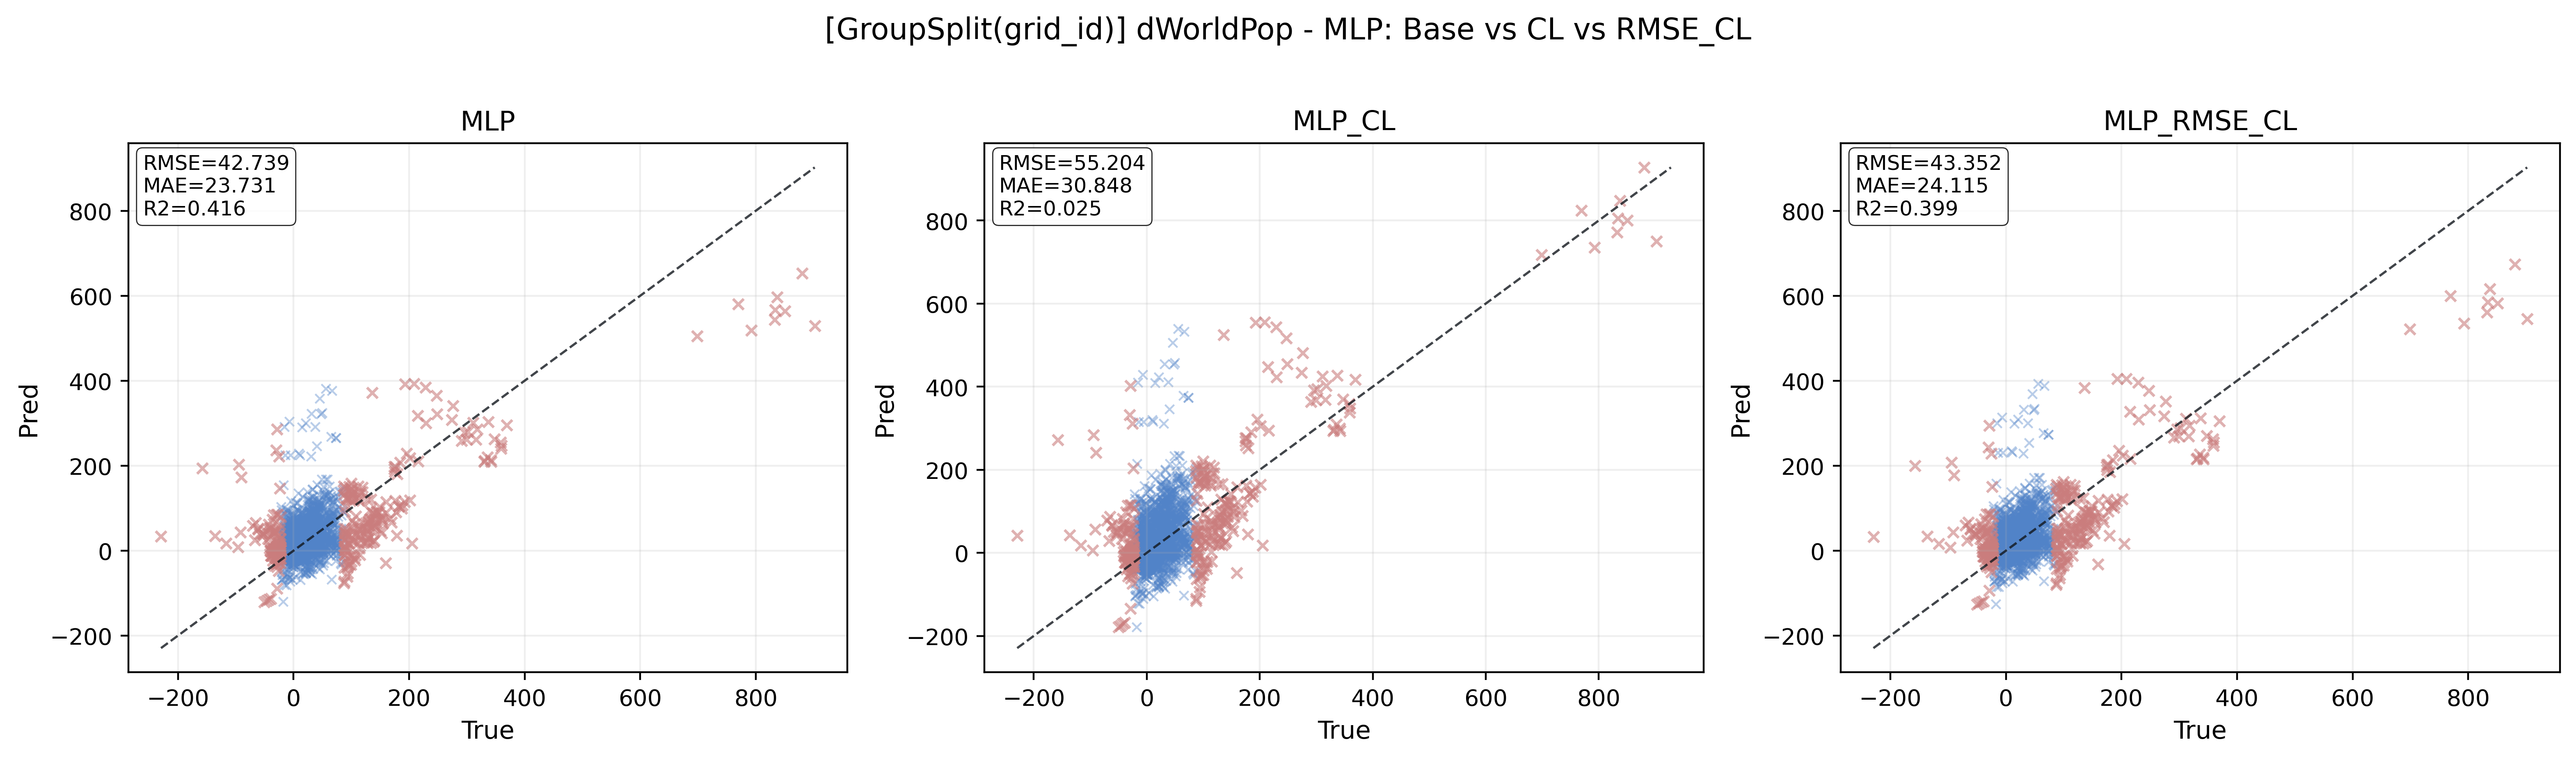
\includegraphics[width=0.98\linewidth]{figures/GroupSplit_grid_id___dWorldPop__MLP__triplet.png}
    \caption{Visualization of contrastive learning adjustment: a representative example showing how contrastive learning improves predictions for tail samples. In the middle graph (MLP\_CL), an upper-right cluster of tail sample predictions improves substantially, while body predictions are stretched by the adjusting layer, leading to a decrease in overall performance.}
    \label{fig:clvisualize}
\end{figure*}





\subsection{Spike Diagnostics and Error Analysis}

We further examine why the calibrator helps. Figure~\ref{fig:clvisualize} shows that calibration mainly changes the geometry of tail predictions rather than uniformly shifting the whole cloud. Tail samples in the upper-right region move closer to the diagonal, indicating that the base model had been systematically conservative on large positive changes. This is a common failure mode in long-tail regression: when rare shocks are underrepresented, the fitted model prefers safer predictions near the center of the distribution.

At the same time, the figure also reveals the main risk of aggressive contrastive adjustment: some body predictions are pulled away from the diagonal. This is why anchoring matters. With the mixed objective, the calibrator can correct tail shrinkage while the RMSE term discourages unnecessary movement of already well-predicted body samples. In other words, the affine layer works not because it is expressive, but because it provides a controlled correction to a recurrent bias in the base predictors.

\textbf{Summary:} the calibration gains are consistent with a simple mechanism: rare extremes are systematically underfit, and a lightly constrained post-hoc layer can correct that bias as long as it remains anchored to pointwise accuracy.

\subsection{Ablations (CL Calibration)}

We evaluate how the mix weight changes the calibration behavior. Empirically, a setting around 5\% RMSE and 95\% CL provides the best trade-off: larger RMSE weights reduce the tail-focused effect, while removing RMSE entirely makes the calibrator unstable. This supports the view that the method succeeds not by replacing standard regression objectives, but by supplementing them with a tail-sensitive correction.

Some models, especially Extra Trees and stronger Random Forest variants, show only modest gains. This is not a contradiction. When a baseline already captures much of the target scale and nonlinearity, the remaining errors are less systematic and therefore less correctable by a one-dimensional affine map. The calibrator is most valuable when there is a persistent tail bias to correct.

\subsection{MoE: Negative Results}

We next test the competing hypothesis that tail robustness should be addressed by routing-based decomposition. In principle, a Mixture-of-Experts should help if tail and body samples correspond to separable regimes with distinct predictive mechanisms. In our setting, however, the opposite occurs.

Table~\ref{tab:dwp_gs_moe_drop} shows that the two-expert MoE under GroupSplit on $\Delta$WorldPop degrades performance relative to a single XGBoost baseline across all metrics:

\begin{table}[htbp]
\centering
\small
\setlength{\tabcolsep}{5pt}
\renewcommand{\arraystretch}{1.10}
\caption{MoE performance degradation on $\Delta$WorldPop, GroupSplit(grid\_id). For $R^2$: gain $= (\text{MoE}-\text{Base})/\text{Base} \times 100\%$ (higher is better). For RMSE: gain $= (\text{Base}-\text{MoE})/\text{Base} \times 100\%$ (higher is better). Negative values indicate degradation.}
\label{tab:dwp_gs_moe_drop}
\begin{tabular}{lrrr}
\toprule
\textbf{Metric} & \textbf{Base} & \textbf{MoE} & \textbf{Gain (\%)} \\
\midrule

\multicolumn{4}{c}{\textbf{Base (XGB) vs.\ MoE (2-expert)}} \\
\cmidrule(lr){1-4}
$R^2_{\mathrm{all}}$    & 0.527   & $0.420$  & $-20.30\%$ \\
RMSE$_{\mathrm{all}}$   & 38.462  & $46.474$   & $-20.83\%$ \\
$R^2_{\mathrm{tail}}$   & 0.563   & $0.321$  & $-42.98\%$ \\
RMSE$_{\mathrm{tail}}$  & 108.125 & $137.703$  & $-27.35\%$ \\

\bottomrule
\end{tabular}
\end{table}

This result is informative rather than incidental. The MoE introduces a harder subproblem than the original regression task: it must first infer whether a sample belongs to the tail regime before either expert can help. Under spatial shift, that routing decision is weakly identifiable from the available features. Figure~\ref{fig:gatingscatter} shows broad ambiguity near the decision boundary, where many samples receive intermediate routing probabilities rather than confident assignments. For a remote-sensing application, this means the model struggles to decide when an observation should be interpreted as an exceptional local change rather than ordinary variability.

Three mechanisms likely drive the degradation. First, routing errors are expensive because the tail regime is rare and mistakes on extreme samples dominate RMSE$_{\text{tail}}$. Second, splitting the data between experts reduces effective sample size, which is especially harmful for a scarce tail regime. Third, the signed-log transformation used for the tail expert may stabilize training locally, but its inverse magnifies small prediction errors when mapped back to the original scale. As a result, the added complexity does not improve specialization; it amplifies instability.

\begin{figure}[htbp]
    \centering
    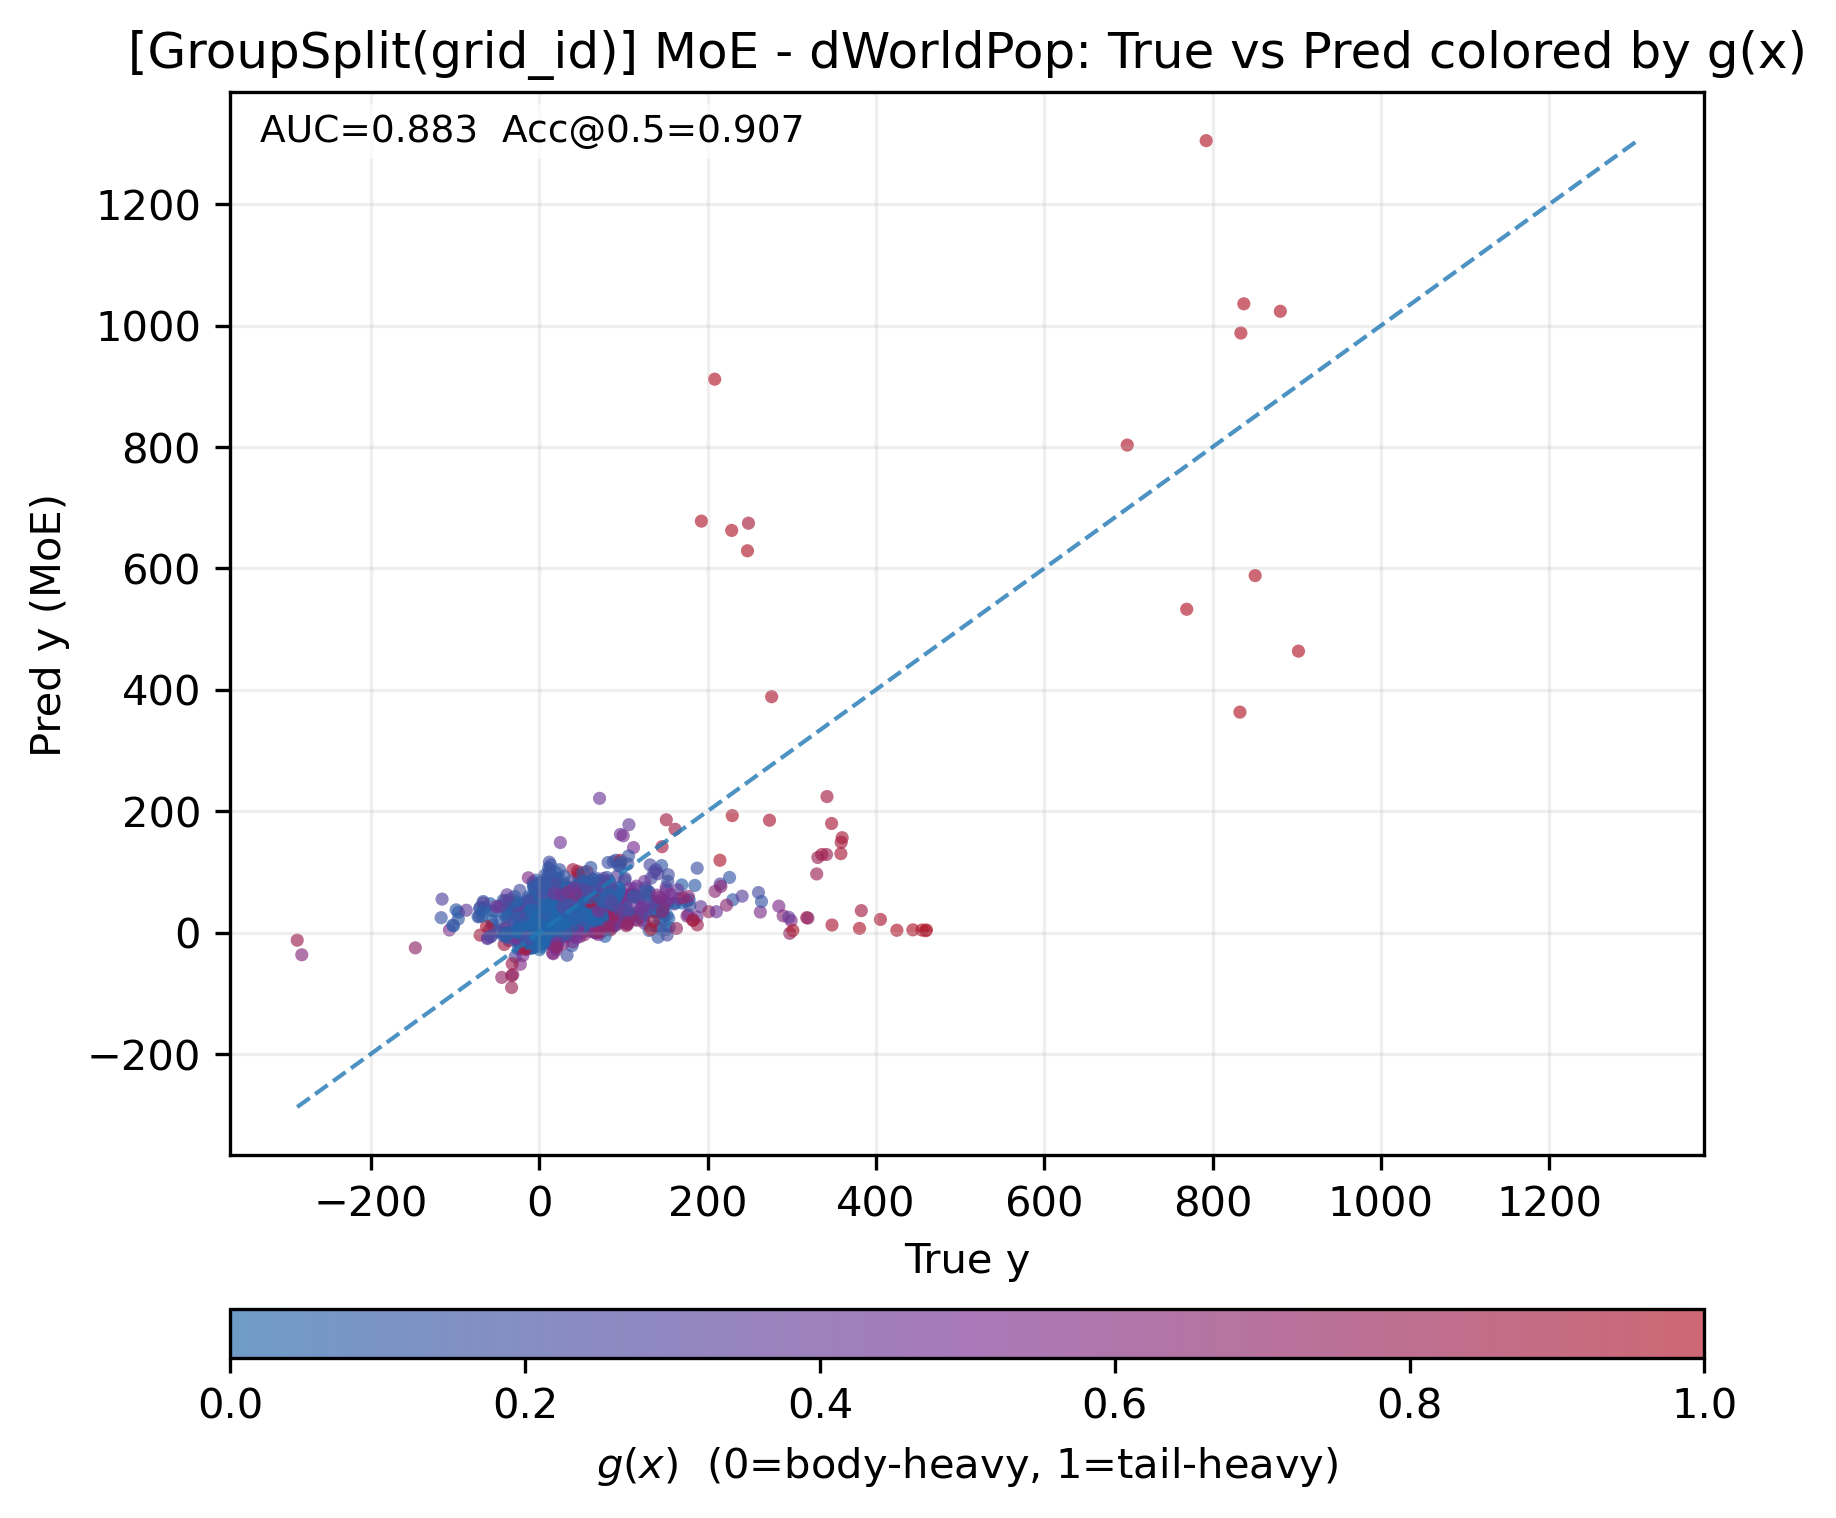
\includegraphics[width=0.9\linewidth]{figures/GroupSplit_grid_id___dWorldPop__MoE__gating_scatter.png}
    \caption{Gating network scatter plots showing the distribution of soft routing probabilities. The gating network attempts to differentiate body and tail samples but exhibits weak separability near the decision boundary, leading to ambiguous expert assignments.}
    \label{fig:gatingscatter}
\end{figure}

% =====================================================
\section{Discussion}

We evaluated machine learning models for predicting population and nighttime luminosity changes using CivitasGrid-TLP. From an applied remote-sensing perspective, the central result is that reliability under spatial transfer matters more than optimistic average performance under permissive splits. RMSE-anchored contrastive calibration substantially improves tail performance without sacrificing overall accuracy, whereas the two-expert MoE unexpectedly underperformed. We also found that $\Delta$VIIRS is substantially more challenging to predict than $\Delta$WorldPop, likely reflecting increased noise from differencing. We discuss these findings in detail below.

\subsection{Cross-Target Performance Differences}

$\Delta$WorldPop predictions consistently outperform $\Delta$VIIRS across all models and metrics. Multiple factors explain this difference. First, nighttime light data generally contain more uncertainty and noise from atmospheric conditions, sensor degradation, and local lighting policies, whereas population data exhibit more stable patterns. Second, year-to-year differencing amplifies noise, which is particularly problematic for VIIRS because it is already noisy. Third, our transportation morphology features may be more informative for population changes than for light intensity changes, suggesting potential benefit from target-specific feature engineering. In other words, the two targets occupy different positions on the remote-sensing signal-to-noise spectrum, and they should not be expected to respond equally well to the same modeling strategy.

\subsection{RMSE+CL Calibration: Mechanisms and Evidence}

The RMSE+CL mixed objective delivers consistent tail improvements. We attribute this to three mechanisms that are especially relevant when remote-sensing proxy products are used for change-focused mapping:

\subsubsection{Anchoring}
The RMSE component prevents the contrastive loss from over-emphasizing tail samples at the expense of body accuracy. By normalizing both terms and weighting them at 5\% RMSE and 95\% CL, the calibrator avoids the instability observed with CL-only (which frequently collapsed overall $R^2$ to negative values in Table~\ref{tab:cl_wide_blocks}).

\subsubsection{Dual Optimization}
RMSE minimization preserves pointwise accuracy while contrastive learning encourages separation between predictions and incorrect targets. This naturally pushes tail predictions (far from the mean) along the regression line, improving reliability without harming body predictions.

\subsubsection{Empirical Evidence}
Under GroupSplit on $\Delta$WorldPop, RMSE+CL achieves a $+69.68\%$ average tail $R^2$ gain while changing overall RMSE by only $-1.94\%$ (Table~\ref{tab:dwp_gs_avg_gain}). This asymmetry shows effective rebalancing toward rare events without degradation. In contrast, CL-only sacrifices $-109.59\%$ overall $R^2$ for only $+40.17\%$ tail $R^2$, indicating that pure contrastive learning is too aggressive.

\subsection{MoE Failure Analysis}

The two-expert MoE underperforms across both overall and tail metrics, highlighting challenges for routing-based approaches in long-tail settings.

First, predicting tail membership from available features is intrinsically difficult: the gating network struggles near quantile thresholds, where samples are inherently ambiguous. Small feature changes can flip expert assignments, amplifying variance and creating boundary artifacts. Second, misrouting is costly: routing a tail sample to the body expert (or vice versa) produces much larger errors than single-model baselines, which is especially problematic when rare extremes dominate tail metrics. Third, while the signed-log transformation stabilizes tail expert training, the inverse transformation magnifies small errors into large absolute values for extreme predictions.

These findings indicate that simple binary MoE with soft/hard gating is ill-suited for this task. More robust approaches---uncertainty-aware gating, continuous mixtures, or threshold-aware routing---may better handle the ambiguity and high stakes of long-tail routing in Earth-observation settings.

\subsection{Practical Recommendations}

For long-tailed targets where tail reliability is critical, we recommend adding a post-hoc RMSE+CL calibration layer to strong baselines such as XGBoost or Random Forest. This lightweight, model-agnostic approach effectively enhances tail predictions while preserving overall performance, making it practical for remote-sensing practitioners who need geographically transferable urban proxy maps rather than only strong in-sample scores.

\subsection{Limitations and Future Work}

We acknowledge several limitations and offer practical directions for future work:

(1) \textit{VIIRS} prediction remains unsatisfactory. Future work should explore smoothed targets (e.g., three-year trends) to reduce differencing noise, suppress transient illumination effects, and improve signal.

(2) Our model predicts point estimates without uncertainty. Quantile regression or Bayesian approaches could enable uncertainty-aware prediction, improving decision support for remote-sensing monitoring workflows.

(3) MoE's failure may stem from weak gating networks. Future work should explore uncertainty-aware or threshold-informed routing mechanisms.

(4) Spatial bias from OSM coverage differences could be mitigated through coverage-weighted training or post-hoc bias correction.

% =====================================================
\section{Conclusion}

Urban proxy dynamics are strongly heavy-tailed: most grid-year changes remain near zero, while rare shocks dominate error and risk. To study this regime reproducibly, we introduced CivitasGrid-TLP, a grid-level panel dataset (2015--2024) that integrates OSM transportation morphology with proxy socioeconomic signals (WorldPop and VIIRS). Framed as an applied remote-sensing task, the dataset supports evaluation of how well models can transfer urban proxy mapping to unseen grids rather than simply interpolate within previously observed locations. We evaluated models under both random splitting (potentially optimistic) and a leakage-resistant GroupSplit(grid\_id) protocol.

Key findings across baselines: $\Delta$WorldPop is substantially more predictable than $\Delta$VIIRS, whose year-to-year differencing amplifies measurement noise, yielding near-zero $R^2$ for most methods. For long-tail robustness, our primary contribution is demonstrating that a lightweight, model-agnostic post-hoc affine calibrator trained with an \emph{RMSE-anchored contrastive} objective consistently improves tail performance while preserving overall accuracy. Pure contrastive loss optimization is often unstable and severely degrades global fit. We also report a negative result: a two-expert MoE (body expert in original space, tail expert in signed-log space) underperforms a single XGBoost baseline on both overall and tail metrics, likely due to weak tail-routing identifiability and amplified transformation errors.

\textbf{Takeaway:} reliable tail gains require anchoring. For practitioners needing improved tail accuracy in remote-sensing proxy mapping, RMSE-anchored contrastive calibration is a practical, lightweight add-on to strong tabular regressors. Naive tail/body MoE routing can collapse under feature--label ambiguity near quantile boundaries.

Future work should address VIIRS noise (via temporal smoothing or trend targets), incorporate uncertainty quantification (quantile or distributional regression), and explore uncertainty-aware or threshold-informed routing mechanisms to improve mixture-model stability in long-tail remote-sensing settings.


% =====================================================
\section*{Acknowledgments}

The author thanks his family and friends for their support.

I acknowledge the public support, through U.S. taxpayer funding, of NASA/NOAA open Earth observation programs (including VIIRS) that enable research worldwide.

\section*{Declaration of competing interest}
The author declares no competing interests.

\section*{Funding}
This research received no external funding.

\section*{Data availability}
CivitasGrid-TLP is publicly available on Zenodo (DOI\: 10.5281/zenodo.18144416)~\cite{huang_2026_18144416}.

\section*{Code availability}
Code is available from the author upon reasonable request.

\section*{Declaration of generative AI and AI-assisted technologies in the manuscript preparation process}
During the preparation of this work the author used ChatGPT in order to improve language polishing and debug LaTeX issues. After using this tool, the author reviewed and edited the content as needed and takes full responsibility for the content of the published article.
% ===================== REFERENCES ====================
\bibliographystyle{elsarticle-num}
\bibliography{reference}

% ===================== APPENDIX ======================

\appendix
\section{Appendix}

\begin{table}[!h]
\centering
\small
\caption{Hyperparameters used in Contrastive Learning experiments}

\label{tab:hyperparams_cl}
\begin{tabular}{
p{3.2cm}
p{3.6cm}
>{\raggedright\arraybackslash}p{8.2cm}
}
\toprule
\textbf{Component} & \textbf{Hyperparameter} & \textbf{Value} \\
\cmidrule(lr){1-3}


\multirow{3}{*}{Global}
& Random seed & \texttt{SEED=42} \\
& Splitting ratios & \texttt{Train/Val/Test = 70\% / 15\% / 15\%} \\
& Group split & \texttt{GroupShuffleSplit; two-stage: hold out test groups, then split remaining groups into train/val} \\
\addlinespace
\cmidrule(lr){1-3}


\multirow{2}{*}{Tail (for reporting)}
& Tail quantiles & \texttt{q05=0.05, q95=0.95 (computed on train split only)} \\
& Tail mask & \(y \le q_{0.05}\) \texttt{or} \(y \ge q_{0.95}\) \\
\addlinespace
\cmidrule(lr){1-3}


\multirow{6}{*}{Baselines (sklearn)}
& Ridge & \(\alpha=1.0\) \\
& ElasticNet & \(\alpha=1.0\), \texttt{l1\_ratio=0.5, max\_iter=5000, random\_state=42} \\
& SVR (RBF) & \(\!C=10.0,\ \epsilon=0.1\), \texttt{kernel=rbf} \\
& RandomForestRegressor & \texttt{n\_estimators=150, max\_depth=None, min\_samples\_split=2,}\\
& & \texttt{min\_samples\_leaf=1, random\_state=42, n\_jobs=-1} \\
& ExtraTreesRegressor & \texttt{n\_estimators=300, max\_depth=None, min\_samples\_split=2,}\\
& & \texttt{min\_samples\_leaf=1, random\_state=42, n\_jobs=-1} \\
& MLPRegressor & \texttt{hidden\_layer\_sizes=(128,64), activation=relu, early\_stopping=True,}\\
& & \texttt{validation\_fraction=0.1, n\_iter\_no\_change=15} \\
\addlinespace
\cmidrule(lr){1-3}


\multirow{11}{*}{CL calibrator (affine)}
& Calibrator form & \(\tilde{y}=a\hat{y}+b\) \texttt{(trainable a,b)} \\
& Mode & \texttt{cl (contrastive-only) or rmse\_cl (mixed)} \\
& CL batch size & \texttt{CL\_BATCH\_SIZE=128} \\
& Epochs & \texttt{CL\_EPOCHS=40} \\
& Learning rate & \texttt{CL\_LR=0.05} \\
& Temperature & \(T=\max(\mathrm{Std}(y_{\mathrm{train}})\cdot \mathrm{CL\_TEMP\_FACTOR},\,10^{-3})\), \texttt{CL\_TEMP\_FACTOR=1.0} \\
& Numerical eps (loss) & \texttt{CL\_EPS=1e-12} \\
& Mixed-loss weights & \texttt{rmse\_weight=0.05, cl\_weight=0.95} \\
& Normalization (rmse0) & \texttt{rmse0 = RMSE on train with initial (a,b)=(1,0)} \\
& Normalization (cl0) & \texttt{Subsample estimate: CL0\_MAX\_N=3000, CL0\_BATCH=512} \\
& Adam update eps & \texttt{eps=1e-8} \\
\bottomrule
\end{tabular}
\end{table}




\end{document}
